\documentclass[]{book}
\usepackage{lmodern}
\usepackage{amssymb,amsmath}
\usepackage{ifxetex,ifluatex}
\usepackage{fixltx2e} % provides \textsubscript
\ifnum 0\ifxetex 1\fi\ifluatex 1\fi=0 % if pdftex
  \usepackage[T1]{fontenc}
  \usepackage[utf8]{inputenc}
\else % if luatex or xelatex
  \ifxetex
    \usepackage{mathspec}
  \else
    \usepackage{fontspec}
  \fi
  \defaultfontfeatures{Ligatures=TeX,Scale=MatchLowercase}
\fi
% use upquote if available, for straight quotes in verbatim environments
\IfFileExists{upquote.sty}{\usepackage{upquote}}{}
% use microtype if available
\IfFileExists{microtype.sty}{%
\usepackage{microtype}
\UseMicrotypeSet[protrusion]{basicmath} % disable protrusion for tt fonts
}{}
\usepackage[margin=1in]{geometry}
\usepackage{hyperref}
\hypersetup{unicode=true,
            pdftitle={Applied Missing data analysis with SPSS and R(Studio)},
            pdfauthor={Martijn Heymans and Iris Eekhout},
            pdfborder={0 0 0},
            breaklinks=true}
\urlstyle{same}  % don't use monospace font for urls
\usepackage{natbib}
\bibliographystyle{apalike}
\usepackage{color}
\usepackage{fancyvrb}
\newcommand{\VerbBar}{|}
\newcommand{\VERB}{\Verb[commandchars=\\\{\}]}
\DefineVerbatimEnvironment{Highlighting}{Verbatim}{commandchars=\\\{\}}
% Add ',fontsize=\small' for more characters per line
\usepackage{framed}
\definecolor{shadecolor}{RGB}{248,248,248}
\newenvironment{Shaded}{\begin{snugshade}}{\end{snugshade}}
\newcommand{\KeywordTok}[1]{\textcolor[rgb]{0.13,0.29,0.53}{\textbf{#1}}}
\newcommand{\DataTypeTok}[1]{\textcolor[rgb]{0.13,0.29,0.53}{#1}}
\newcommand{\DecValTok}[1]{\textcolor[rgb]{0.00,0.00,0.81}{#1}}
\newcommand{\BaseNTok}[1]{\textcolor[rgb]{0.00,0.00,0.81}{#1}}
\newcommand{\FloatTok}[1]{\textcolor[rgb]{0.00,0.00,0.81}{#1}}
\newcommand{\ConstantTok}[1]{\textcolor[rgb]{0.00,0.00,0.00}{#1}}
\newcommand{\CharTok}[1]{\textcolor[rgb]{0.31,0.60,0.02}{#1}}
\newcommand{\SpecialCharTok}[1]{\textcolor[rgb]{0.00,0.00,0.00}{#1}}
\newcommand{\StringTok}[1]{\textcolor[rgb]{0.31,0.60,0.02}{#1}}
\newcommand{\VerbatimStringTok}[1]{\textcolor[rgb]{0.31,0.60,0.02}{#1}}
\newcommand{\SpecialStringTok}[1]{\textcolor[rgb]{0.31,0.60,0.02}{#1}}
\newcommand{\ImportTok}[1]{#1}
\newcommand{\CommentTok}[1]{\textcolor[rgb]{0.56,0.35,0.01}{\textit{#1}}}
\newcommand{\DocumentationTok}[1]{\textcolor[rgb]{0.56,0.35,0.01}{\textbf{\textit{#1}}}}
\newcommand{\AnnotationTok}[1]{\textcolor[rgb]{0.56,0.35,0.01}{\textbf{\textit{#1}}}}
\newcommand{\CommentVarTok}[1]{\textcolor[rgb]{0.56,0.35,0.01}{\textbf{\textit{#1}}}}
\newcommand{\OtherTok}[1]{\textcolor[rgb]{0.56,0.35,0.01}{#1}}
\newcommand{\FunctionTok}[1]{\textcolor[rgb]{0.00,0.00,0.00}{#1}}
\newcommand{\VariableTok}[1]{\textcolor[rgb]{0.00,0.00,0.00}{#1}}
\newcommand{\ControlFlowTok}[1]{\textcolor[rgb]{0.13,0.29,0.53}{\textbf{#1}}}
\newcommand{\OperatorTok}[1]{\textcolor[rgb]{0.81,0.36,0.00}{\textbf{#1}}}
\newcommand{\BuiltInTok}[1]{#1}
\newcommand{\ExtensionTok}[1]{#1}
\newcommand{\PreprocessorTok}[1]{\textcolor[rgb]{0.56,0.35,0.01}{\textit{#1}}}
\newcommand{\AttributeTok}[1]{\textcolor[rgb]{0.77,0.63,0.00}{#1}}
\newcommand{\RegionMarkerTok}[1]{#1}
\newcommand{\InformationTok}[1]{\textcolor[rgb]{0.56,0.35,0.01}{\textbf{\textit{#1}}}}
\newcommand{\WarningTok}[1]{\textcolor[rgb]{0.56,0.35,0.01}{\textbf{\textit{#1}}}}
\newcommand{\AlertTok}[1]{\textcolor[rgb]{0.94,0.16,0.16}{#1}}
\newcommand{\ErrorTok}[1]{\textcolor[rgb]{0.64,0.00,0.00}{\textbf{#1}}}
\newcommand{\NormalTok}[1]{#1}
\usepackage{longtable,booktabs}
\usepackage{graphicx,grffile}
\makeatletter
\def\maxwidth{\ifdim\Gin@nat@width>\linewidth\linewidth\else\Gin@nat@width\fi}
\def\maxheight{\ifdim\Gin@nat@height>\textheight\textheight\else\Gin@nat@height\fi}
\makeatother
% Scale images if necessary, so that they will not overflow the page
% margins by default, and it is still possible to overwrite the defaults
% using explicit options in \includegraphics[width, height, ...]{}
\setkeys{Gin}{width=\maxwidth,height=\maxheight,keepaspectratio}
\IfFileExists{parskip.sty}{%
\usepackage{parskip}
}{% else
\setlength{\parindent}{0pt}
\setlength{\parskip}{6pt plus 2pt minus 1pt}
}
\setlength{\emergencystretch}{3em}  % prevent overfull lines
\providecommand{\tightlist}{%
  \setlength{\itemsep}{0pt}\setlength{\parskip}{0pt}}
\setcounter{secnumdepth}{5}
% Redefines (sub)paragraphs to behave more like sections
\ifx\paragraph\undefined\else
\let\oldparagraph\paragraph
\renewcommand{\paragraph}[1]{\oldparagraph{#1}\mbox{}}
\fi
\ifx\subparagraph\undefined\else
\let\oldsubparagraph\subparagraph
\renewcommand{\subparagraph}[1]{\oldsubparagraph{#1}\mbox{}}
\fi

%%% Use protect on footnotes to avoid problems with footnotes in titles
\let\rmarkdownfootnote\footnote%
\def\footnote{\protect\rmarkdownfootnote}

%%% Change title format to be more compact
\usepackage{titling}

% Create subtitle command for use in maketitle
\newcommand{\subtitle}[1]{
  \posttitle{
    \begin{center}\large#1\end{center}
    }
}

\setlength{\droptitle}{-2em}

  \title{Applied Missing data analysis with SPSS and R(Studio)}
    \pretitle{\vspace{\droptitle}\centering\huge}
  \posttitle{\par}
    \author{Martijn Heymans and Iris Eekhout}
    \preauthor{\centering\large\emph}
  \postauthor{\par}
      \predate{\centering\large\emph}
  \postdate{\par}
    \date{2018-09-10}

\usepackage{booktabs}

\usepackage{amsthm}
\newtheorem{theorem}{Theorem}[chapter]
\newtheorem{lemma}{Lemma}[chapter]
\theoremstyle{definition}
\newtheorem{definition}{Definition}[chapter]
\newtheorem{corollary}{Corollary}[chapter]
\newtheorem{proposition}{Proposition}[chapter]
\theoremstyle{definition}
\newtheorem{example}{Example}[chapter]
\theoremstyle{definition}
\newtheorem{exercise}{Exercise}[chapter]
\theoremstyle{remark}
\newtheorem*{remark}{Remark}
\newtheorem*{solution}{Solution}
\begin{document}
\maketitle

{
\setcounter{tocdepth}{1}
\tableofcontents
}
\chapter*{Preface}\label{preface}
\addcontentsline{toc}{chapter}{Preface}

The attention for missing data is growing and so will be the application
of methods to solve the missing data problem. From our experience,
researchers with missing data still find it difficult to reserve time to
evaluate the missing data and from that to find a reasonable solution to
handle their missing data for their main data analysis. This manual is
developed for researchers that are looking for a solution of their
missing data problem or want to learn more about missing data. The
manual is developed as a result of a missing data course that we give.
Further, we are also active in providing statistical advice in general
and more specific about missing data. Because our time to give advice is
mostly limited we wanted to give researchers a practical guide to help
them get started with their missing data problem. Leading methodologists
and statisticians and leading journals have published papers about the
problems of missing data and warned researchers to take missing data
seriously (Sterne et al., BMJ 2009, Little et al. NEJM 2012, Peng et al.
2015, JAMA). Hopefully this manual will help researchers to find the
best solution for their missing data problem. We hope you will enjoy
this manual and that you learn from it, at least to take missing data
seriously and that you will use recommended methods to solve your
missing data problem.

\section{The goal of this Manual}\label{the-goal-of-this-manual}

In this manual the software packages SPSS and R play a central role. The
combination of these two software packages may seem a coincidence, but
it is not. For a long time, SPSS was the most popular software package
worldwide to do statistical data analysis. Currently, R is growing in
popularity fast and will probably become one of the most popular
Software packages to do data analysis. Also for applied researchers.
Both SPSS and R have their advantages and disadvantages. An advantage of
SPSS is that it is a user-friendly software package compared to R and
works with windows where you can for example drag your variables to.
Subsequently, you can click the OK button and the statistical analysis
procedure you prespecified gives you the output results. A disadvantage
of SPSS may be that you are overloaded with statistical output that may
not all needed to answer your research question. Compared to SPSS you
could say that R is a more user-unfriendly software package where you
need to use R code to activate statistical procedures and to get
statistical results. R output will show more specific results, without
extra information. Furthermore, R works much faster when it comes to
running statistical procedures by using 1 or 2 lines of R code, compared
to visiting a couple of windows in SPSS to activate the same statistical
test. There is one other advantage of R and that is, that it is open
source. This makes it possible for applied researchers to follow the
calculations of complex procedures as the estimation of missing values
closely along the line. You could say that R brings you to the heart of
the matter. With R it is possible to turn complex data analysis
functions and formula´s into computer code that can be used by everybody
and vice versa. Because it is open source, you are able to read the code
that is used for the analysis and to relate that code or pieces of code
to the statistical output. This makes it possible to evaluate step by
step the code and thus the statistical procedures and relate them to the
subsequent results. You can copy specific parts of code from functions
that others have written and evaluate what happens. This is one of the
major advantages of R if you compare it to the closed source statistical
package SPSS. R brings you a big learning environment when it comes to
the understanding of all kind of statistical procedures as missing data
analysis.

\section{Multiple Imputation in SPSS and
R}\label{multiple-imputation-in-spss-and-r}

Multiple Imputation (MI) is a procedure that is developed in the 1970's
by Donald Rubin. Later, around the 1990´s Multiple imputation was
further developed and became more popular. For a long time, MI was only
available for S-Plus and R software (S-plus is the commercial
alternative of R), where it was further developed by Stef van Buuren, a
statistician from TNO, Leiden, The Netherlands. For a long time, it was
not possible to do MI analysis in SPSS because it was not available in
SPSS. So, it was far out of reach for applied researchers for a long
time. It became available from SPSS version 17. From that time MI is now
used more by applied researchers. In this manual the handling of missing
data is the main topic. We will also show how to apply these methods in
both software packages SPSS and R. To apply the imputation methods that
are discussed both software packages make use of random starting
procedures. SPSS and R use for that intern random number generators.
Because these are different, result might slightly differ. Our intention
is not to compare the software packages SPSS and R and their output
resultys. Both are trustful packages, it is more the estimation
procedures that might lead to the differences. The imputation methods,
will be applied in SPSS version 24 and with R software version 3.4.3.
The R examples will be presented by using the output from RStudio
version (version 1.1.383 -- © 2009-2017 RStudio, Inc.). RStudio is an
integrated development environment (IDE) for R. RStudio includes a wide
range of productivity enhancing features and runs on all major
platforms. As already stated, R allows you to program the statistical
formula's yourself. We have therefore chosen to explain the formula's in
more detail in combination with the application in R. The more applied
researchers will be satisfied with the explanation and application of
methods in SPSS.

\section{Notation and annotation in this
manual}\label{notation-and-annotation-in-this-manual}

The name of R packages, libraries and functions can be recognized by
using Courier new lettertype, for example the package mice will be
written as mice.

R code of the procedures used in the manual is marked grey and the
explanation in these grey parts can be found in the grey parts itself
annotated by the \# symbol. The lines that start with the symbol
\textgreater{} are R Code lines that have been running in the R Console
in RStudio. Example:

\textbf{R code XX}

\begin{Shaded}
\begin{Highlighting}[]
\CommentTok{# Activate the foreign package and read in the SPSS dataset}

\KeywordTok{library}\NormalTok{(foreign)}
\NormalTok{dataset <-}\StringTok{ }\KeywordTok{read.spss}\NormalTok{(}\DataTypeTok{file=}\StringTok{"data/Backpain 50 missing.sav"}\NormalTok{, }\DataTypeTok{to.data.frame=}\NormalTok{T)}
\end{Highlighting}
\end{Shaded}

\begin{verbatim}
## re-encoding from UTF-8
\end{verbatim}

\chapter{Software applications}\label{software-applications}

Statistical software programs can help us to analyze our data. SPSS and
R are such programs. Although SPSS and R are among the most popular
programs to do statistical data analyses nowadays, they do not have much
in common. One of the greatest differences is that SPSS works with menu
options that make windows appear and you can click buttons to select
options, whereas R works with lines of code that you have to type in to
run analyses. This makes SPSS more user-friendly than R for applied
researchers. In SPSS you are overloaded with output tables, and in R you
only get output on demand. In this Chapter we will explore the different
possibilities of the SPSS (IBM 2016) and the R software language
(Matloff, 2011, Dalgaard, 2008). We will run R via RStudio, the
integrated development environment (IDE) for R. RStudio includes a wide
range of productivity enhancing features, which makes it easier to work
with than with the R console on its own.

\section{SPSS, Data and Variable View
windows}\label{spss-data-and-variable-view-windows}

In this manual we work with SPSS version 24 (IBM, 2016). When you start
SPSS Version 24 a start-up window appears. In this window, you can
directly open the files that were active during your previous use of
SPSS. These files can be found and easily opened in the ``Recent files''
window (Figure \ref{fig:fig1}). If you do not want to see this window
the next time that you open SPSS, select ``Don't show this dialog in the
future''.

\begin{figure}

{\centering 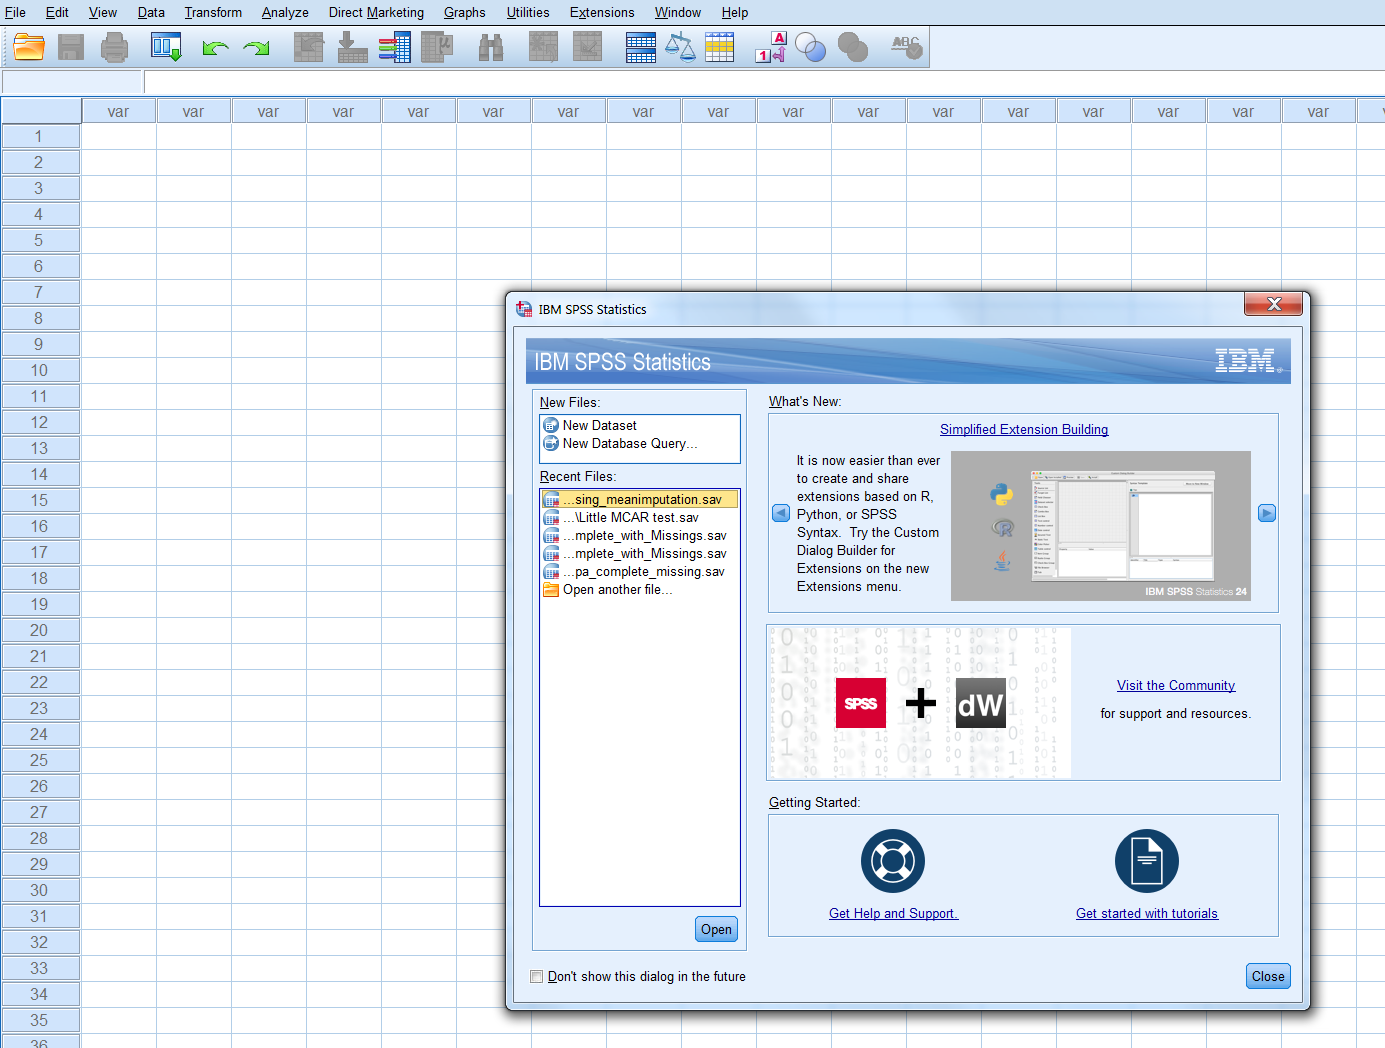
\includegraphics[width=0.9\linewidth]{images/fig1.1} 

}

\caption{First window after you have started SPSS}\label{fig:fig1}
\end{figure}

When you click on Close on the right side below, the window will close
and you will see an empty Data View window. Now you are in the SPSS Data
Editor window. This window is always open when you start SPSS. The name
``SPSS Data Editor'' is also visible at the top of the screen and is
called ``IBM SPSS Statistics Data Editor'' (Figure \ref{fig:fig2}).

\begin{figure}

{\centering 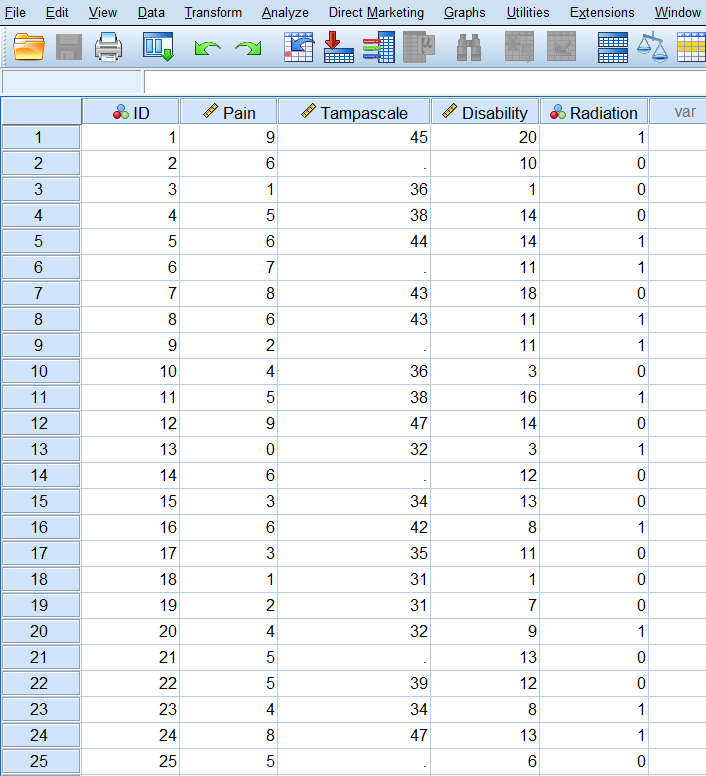
\includegraphics[width=0.9\linewidth]{images/fig1.2} 

}

\caption{Data View window in SPSS}\label{fig:fig2}
\end{figure}

In the SPSS Data Editor, you have the possibility to go to the Data View
and Variable View windows. In the Data View window, you can enter data
yourself or read in data by using the options in the file menu. In
Figure 1.2 you see an example of a dataset in the Data View window. Each
row in the Data View window represents a case and in the columns you
will find the variable names. In the Data View window, you can do all
kind of data manipulations by using the different menu's above in the
window. From here you can click on the tab Variable View, in the lower
left corner of the window. Than the Variable view window will appear
(Figure \ref{fig:fig3}).

\begin{figure}

{\centering 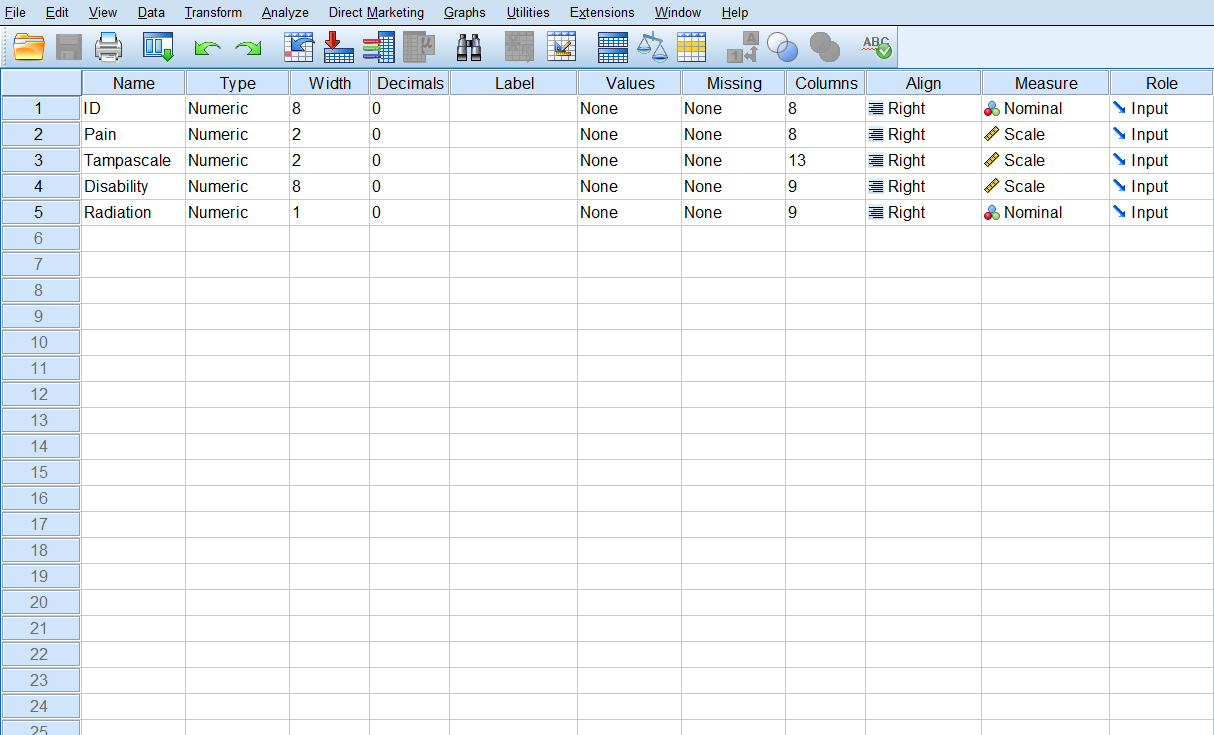
\includegraphics[width=0.9\linewidth]{images/fig1.3} 

}

\caption{Variable View window in SPSS}\label{fig:fig3}
\end{figure}

In the Variable View window, you can add new variables, by entering the
name in the name column. Further, you can change the columns by using
the following options: Type: Here you can change the type of variables
in your dataset. Mostly you work with numeric variables, i.e.~a variable
whose values are numbers. Other possibilities are Date variables which
is a numeric variable whose values are displayed in one of several
calendar-date or clock-time formats or String variables, a character
(text) variable that can contain any characters up to the defined
length. String values are not numeric and therefore are not used in
calculations. Width: By default SPSS defines a numeric variable with 8
digits for each new variable.

Decimals: the number of decimal places displayed.

Label: The variable name.

Values: To assign numbers to the categories of a variable. To define
Variable values do the following: 1. Click the button in the Values cell
for the variable that you want to define. 2. For each value, enter the
value and a label. 3. Click Add to enter the value label. 4. Click OK.

Missing: Here you can define specified data values as user-missing. You
can enter up to three discrete (individual) missing values, a range of
missing values, or a range plus one discrete value.

Columns: To change the number of characters displayed in the Data View
window.

Align: Here you can specify the alignment of your data.

Measure: Here you can specify the level of each variable, scale
(continuous), ordinal or nominal.

Role: Here you can define the role of the variable during your analysis.
Examples are, Input for independent variable, Target for dependent or
outcome variable, Both, independent and dependent variable. There are
more possibilities, but most of the times you use the default Input
setting.

\section{Analyzing data in SPSS}\label{analyzing-data-in-spss}

All statistical procedures in SPSS can be found under the Analyze button
(Figure \ref{fig:fig4}). Here you also will find the option ``Multiple
Imputation'' which plays an important role in this manual. We will use
this menu later on in Chapter 4.

\begin{figure}

{\centering 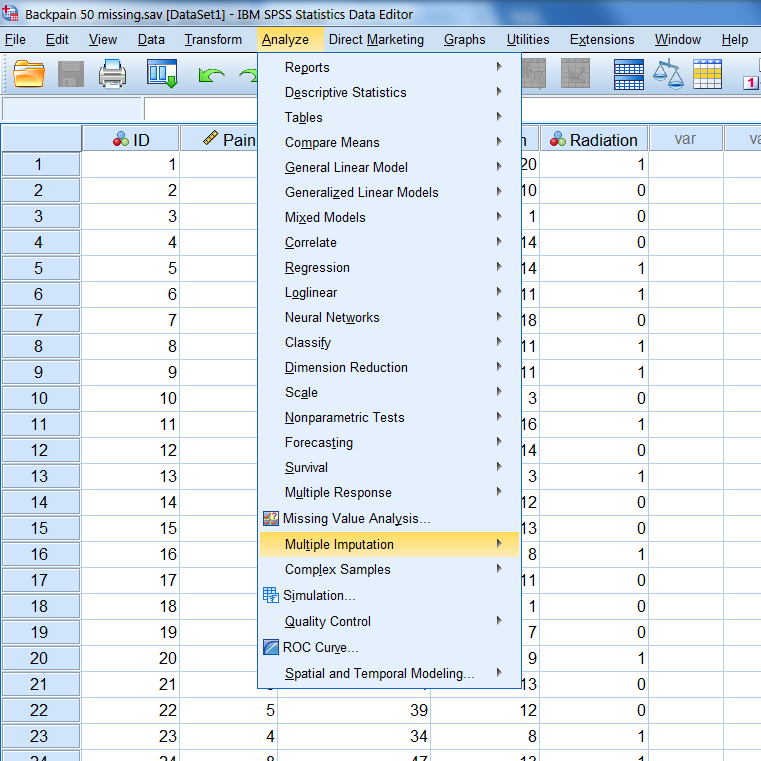
\includegraphics[width=0.9\linewidth]{images/fig1.4} 

}

\caption{Statistical procedures that can be found under the Analyze menu in SPSS}\label{fig:fig4}
\end{figure}

\section{Data Transformations in
SPSS}\label{data-transformations-in-spss}

Two other interesting buttons are Data and Transform. The Data menu
allows you to make changes to the data editor. Here you can add new
variables or cases. You can also use the Split File option, to get
analyses results separately for categories of a variable. The Transform
menu allows you to manipulate your variables by for example
dichotomizing a numeric variable.

\section{The Output window in SPSS}\label{the-output-window-in-spss}

If you have run your analyses in SPSS, an SPSS Output (or viewer) Window
will pop-up. The main body of the Output Window consists of two panes
(left and right panes). In the left pane you will find an outline of the
output. In the right pane you will find the actual output of your
statistical procedure (Figure \ref{fig:fig5}).

\begin{figure}

{\centering 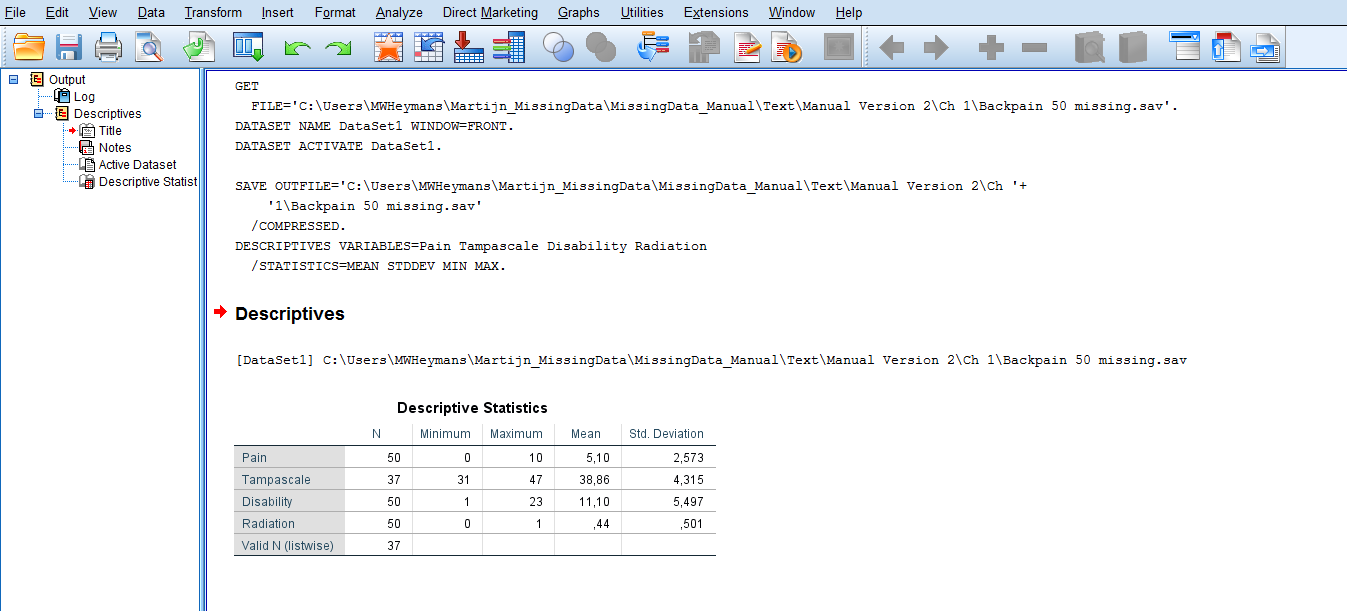
\includegraphics[width=0.9\linewidth]{images/fig1.5} 

}

\caption{Part of the Output or Viewer window in SPSS after making use of Descriptive Statistics under the Analyze menu}\label{fig:fig5}
\end{figure}

\section{The Syntax Editor in SPSS}\label{the-syntax-editor-in-spss}

In the syntax editor of SPSS, you use the SPSS syntax programming
language. You can run all SPSS procedures by typing in commands in this
syntax editor window, instead of using the graphical user interface,
i.e.~by using your mouse and clicking on the menu´s. You can get access
to the syntax window in two ways. The first is just by opening a new
syntax file by navigating to File -\textgreater{} New -\textgreater{}
Syntax. This will open a new syntax window (Figure \ref{fig:fig6}).

\begin{figure}

{\centering 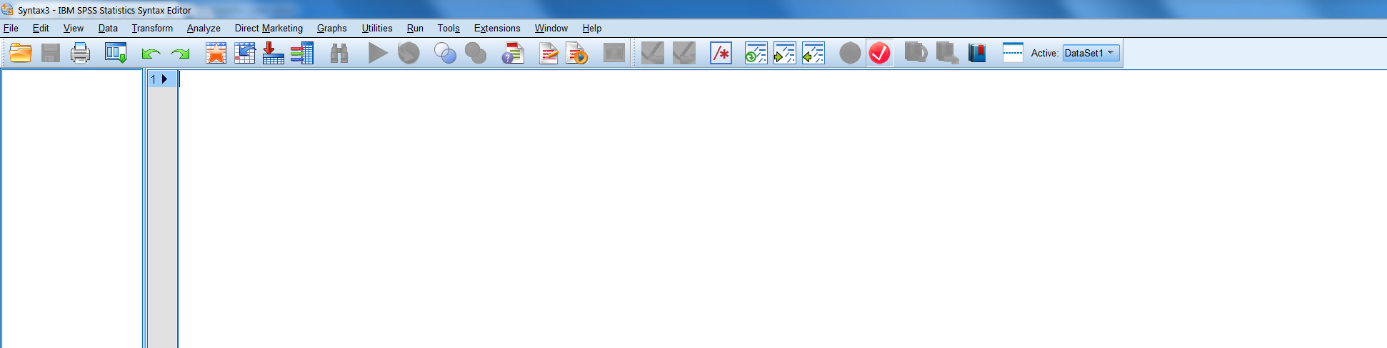
\includegraphics[width=0.9\linewidth]{images/fig1.6} 

}

\caption{Screenshot of new syntax file}\label{fig:fig6}
\end{figure}

Now you can start writing your syntax directly in this window. You can
also generate syntax by accessing statistical procedures through the
dropdown menus and clicking the Paste button instead of clicking the OK
button after you have specified the options. When you have clicked the
Paste button, a new Syntax Editor window will pop up or the new syntax
will automatically be added to the open Syntax Editor window. This is a
very useful way to keep track of the analysis that you have performed.
An example can be found in Figure \ref{fig:fig7}, where the syntax is
shown for the Descriptive Statistics procedure of Figure \ref{fig:fig5}.

\begin{figure}

{\centering 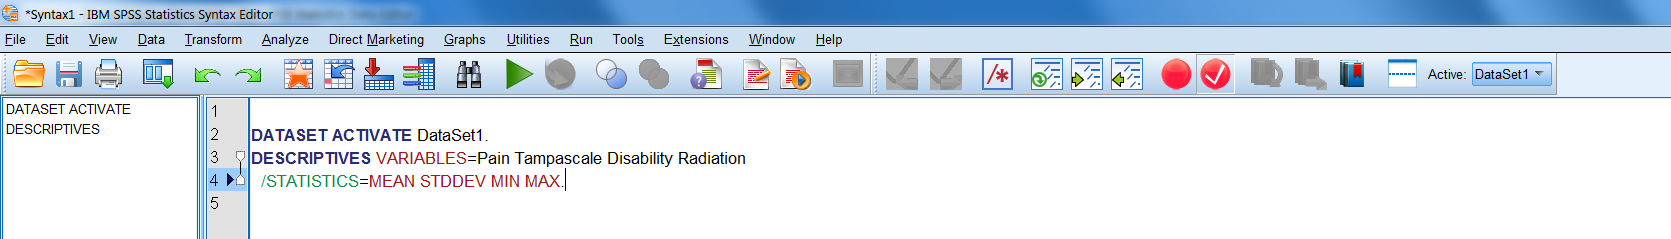
\includegraphics[width=0.9\linewidth]{images/fig1.7} 

}

\caption{Screenshot of Syntax editor of SPSS including the Syntax code for descriptive statisitcs}\label{fig:fig7}
\end{figure}

By using the SPSS Syntax it is possible for users to perform the same
analyses over and over again or to adapt the analysis via the syntax
code for complex calculations in the data. In this manual we will not
use SPSS syntax code to access statistical procedures, however we
recommend to use the SPSS syntax to keep track of the analysis that you
have performed. SPSS is most frequently used via the graphical user
interface, and we will use that method also in this manual.

\section{Reading and saving data in
SPSS}\label{reading-and-saving-data-in-spss}

Reading in data in SPSS is very easy; via the menu File choose for File
-\textgreater{} Open -\textgreater{} Data. All kind of file types can be
selected. Of course the SPSS .sav files, but also .por, .xlsx, .cvs,
SAS, Stata, etc. (Figure 1.8). After you have selected a specific file
type you may have to go through several steps before you see the data in
the Data View window. These steps are not necessary for SPSS files, they
open directly in the data editor.

\begin{figure}

{\centering 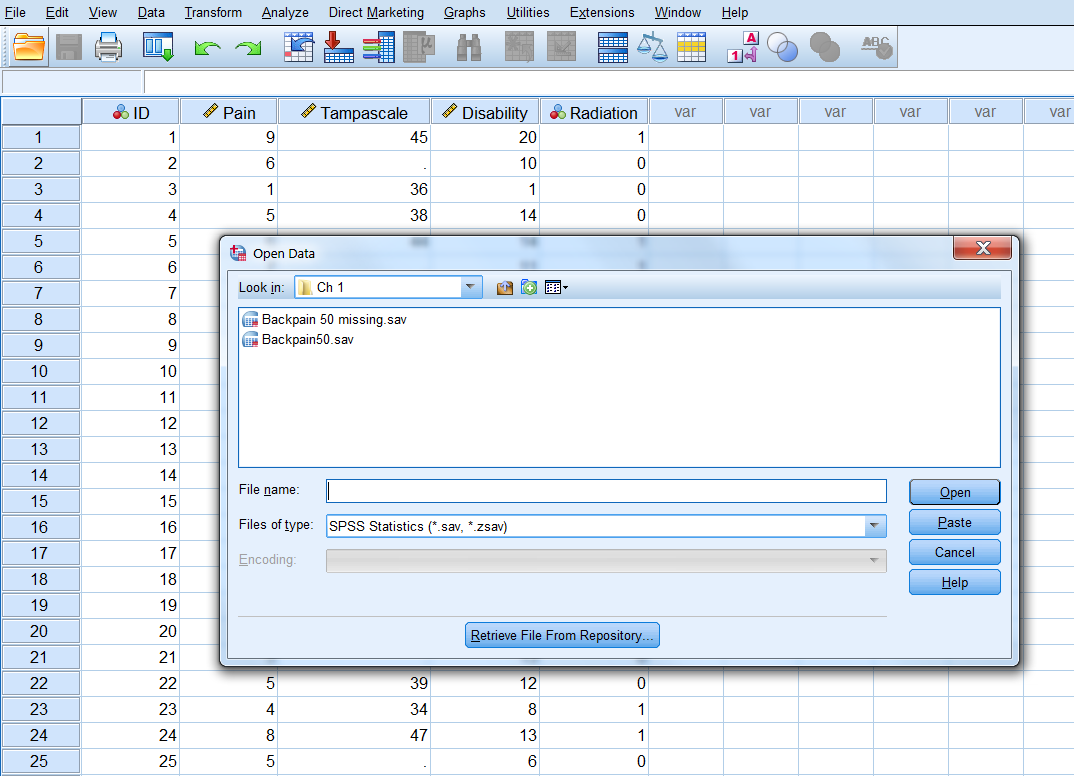
\includegraphics[width=0.9\linewidth]{images/fig1.8} 

}

\caption{Window to read in different file types in SPSS}\label{fig:fig8}
\end{figure}

Saving files in SPSS is possible via the Save Data As option under the
menu File. You can choose the same kind of file types (Figure
\ref{fig:fig9}).

\begin{figure}

{\centering 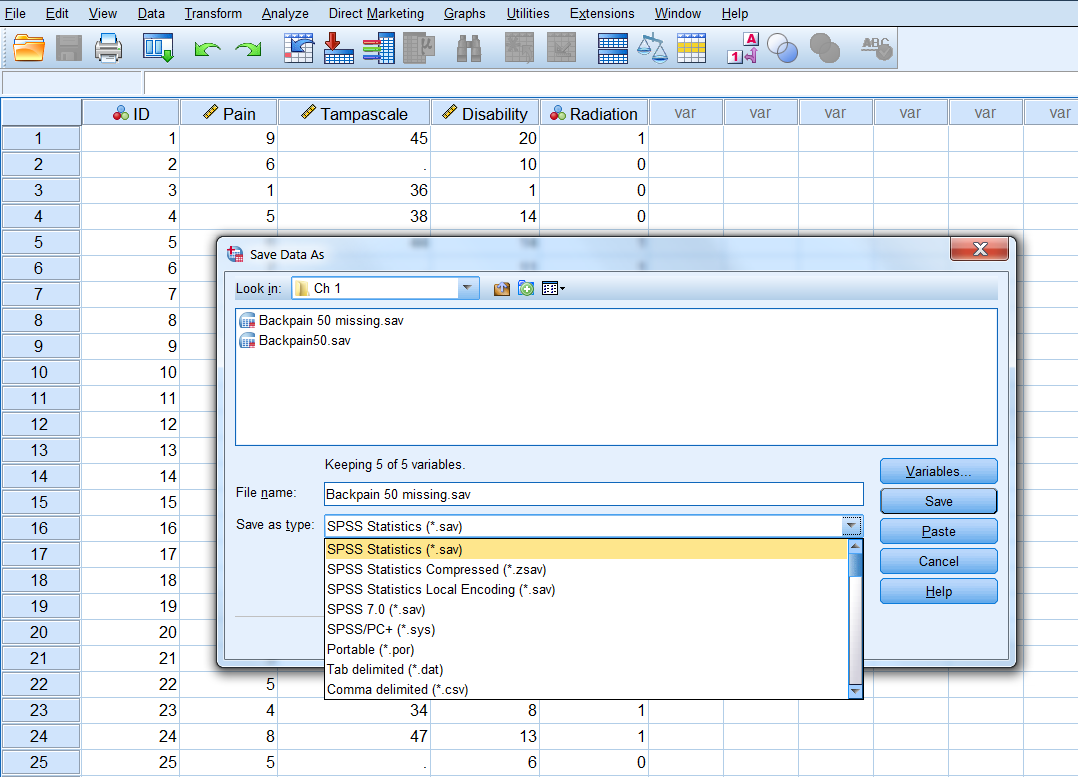
\includegraphics[width=0.9\linewidth]{images/fig1.9} 

}

\caption{Option Save Data As under the menu File}\label{fig:fig9}
\end{figure}

\section{R and RStudio}\label{r-and-rstudio}

RStudio is an integrated environment to work with the software program
R. Consequently, to work with RStudio, R has to be installed. RStudio
uses the R language and is also freely available. In this manual we will
only show some possibilities and options in RStudio that are needed to
run the R code and the programs that are discussed in this manual. For
more information about RStudio and its possibilities visit the RStudio
website at www.rstudio.com. When you open RStudio the following screen
will appear.

\begin{figure}

{\centering 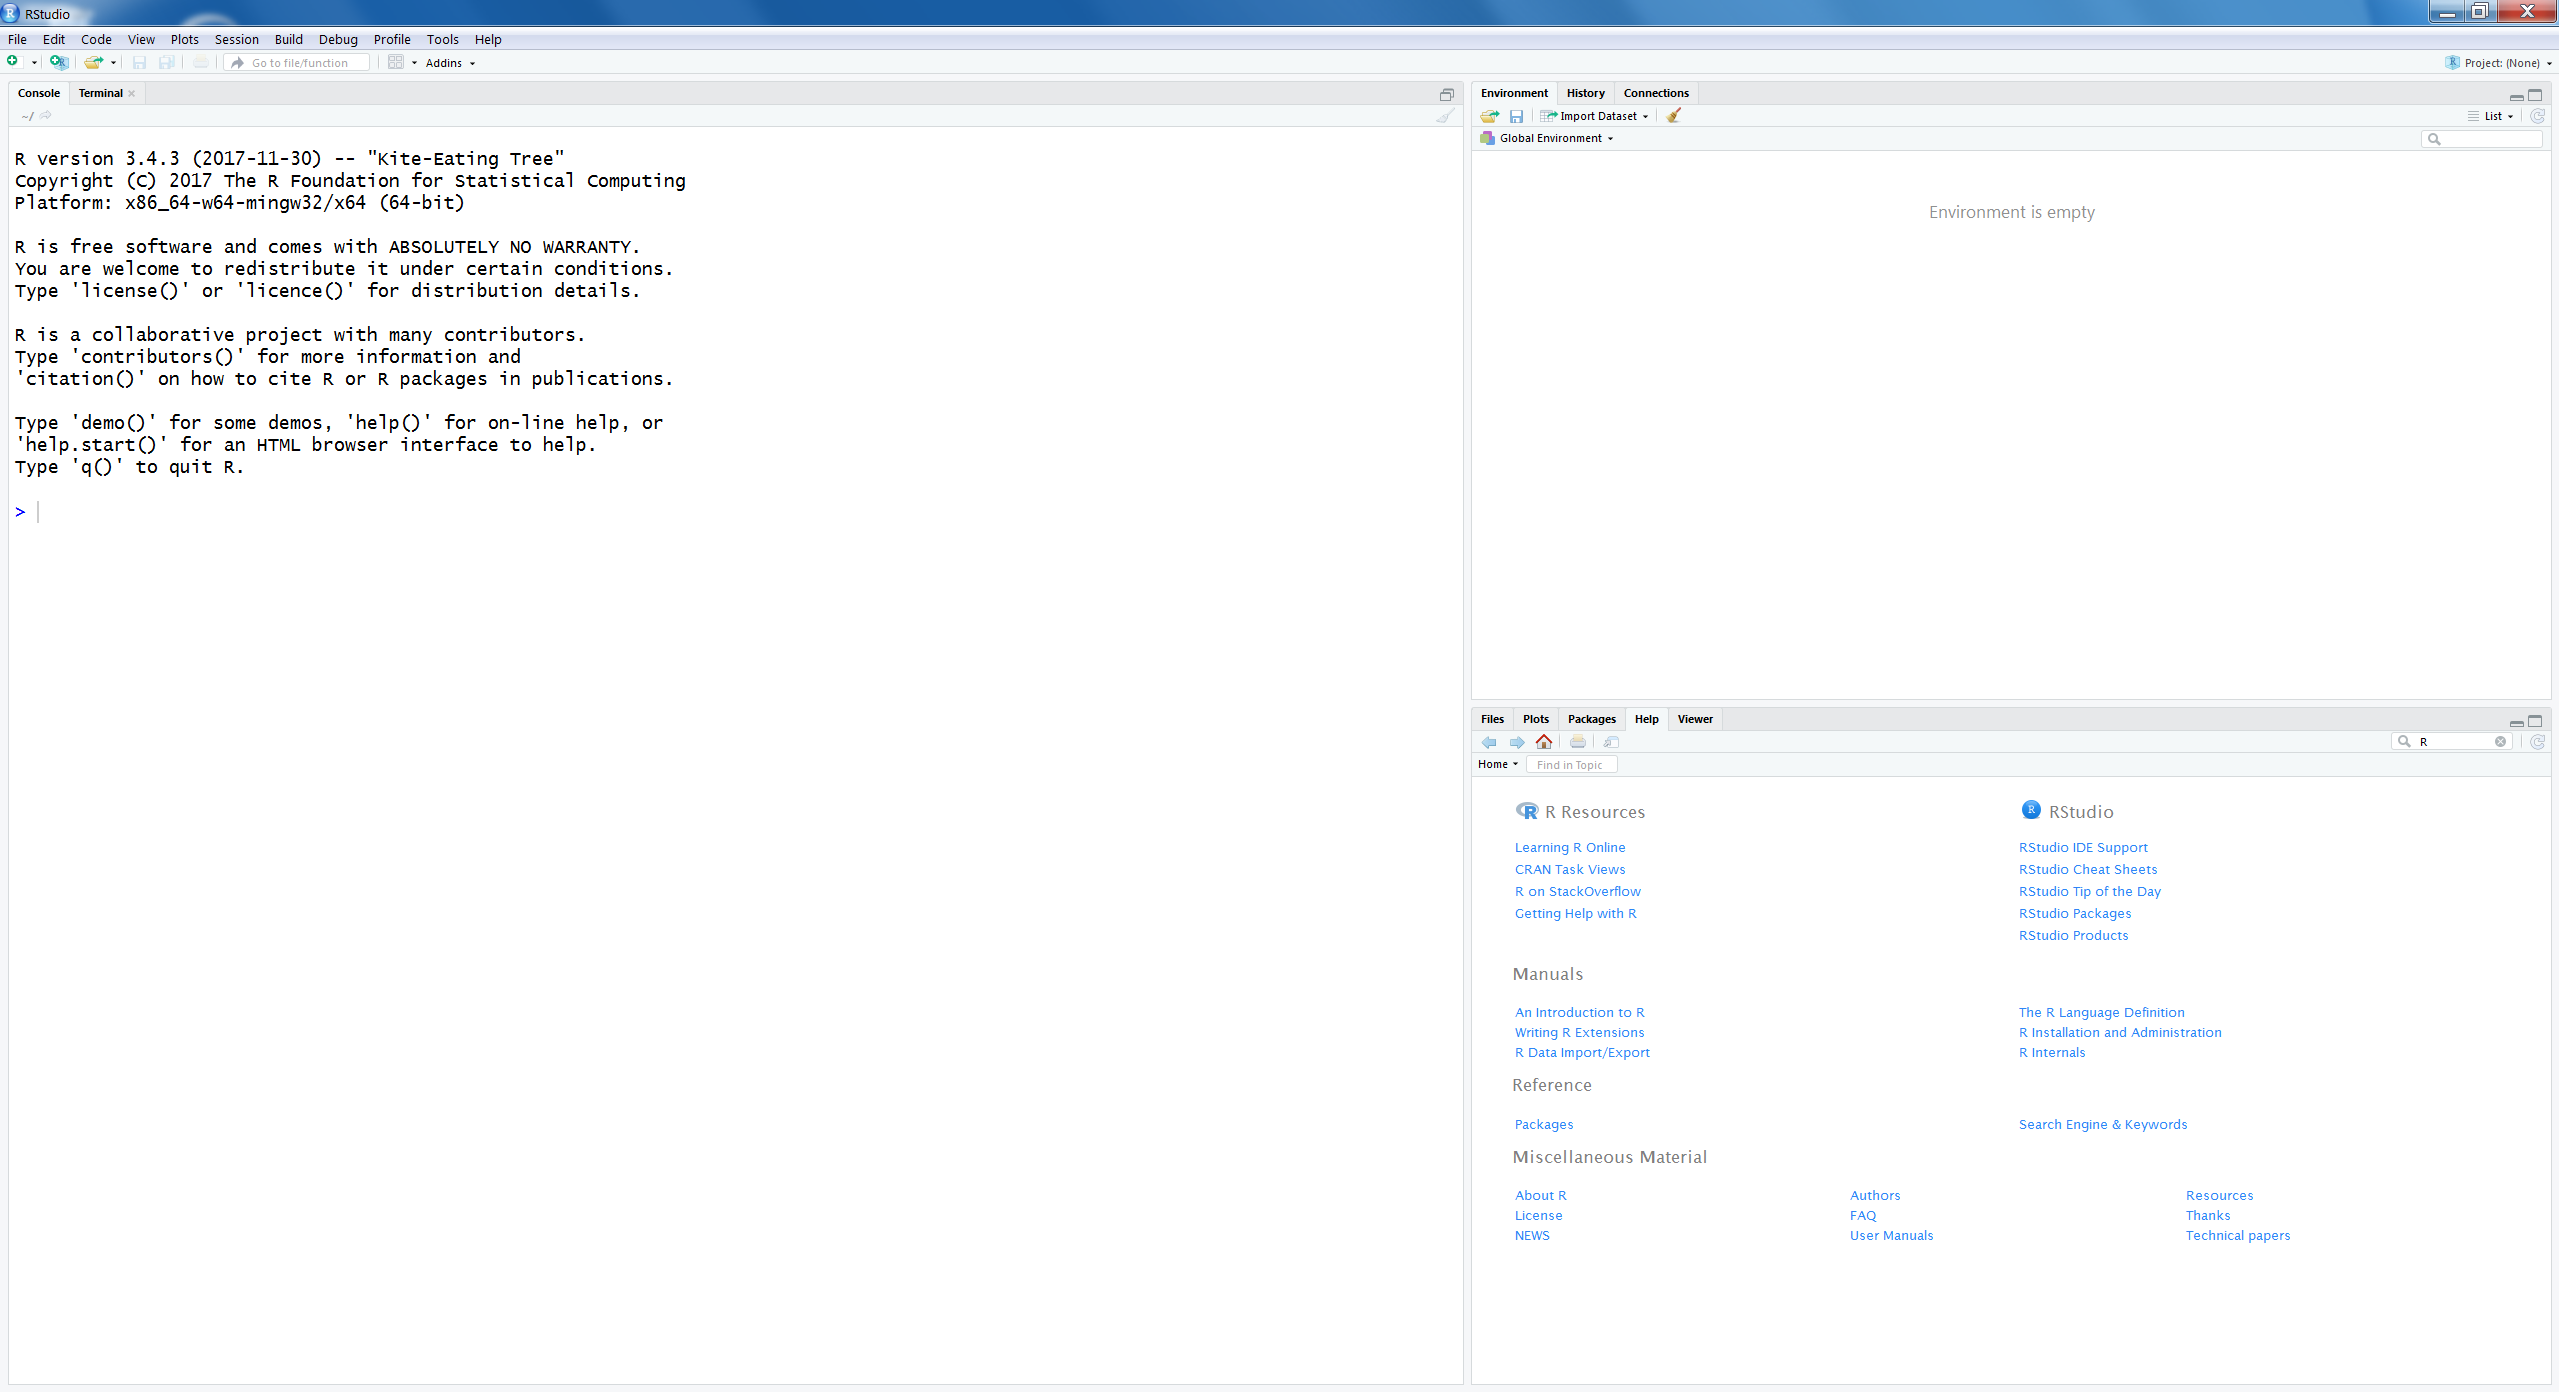
\includegraphics[width=0.9\linewidth]{images/fig1.10} 

}

\caption{First screen that appears after you have started RStudio}\label{fig:fig10}
\end{figure}

There are three windows opened:

\begin{enumerate}
\def\labelenumi{\arabic{enumi}.}
\tightlist
\item
  On the left is the Console window
\end{enumerate}

This is the main window to run R code (see below for more information
about the Console window).

\begin{enumerate}
\def\labelenumi{\arabic{enumi}.}
\setcounter{enumi}{1}
\tightlist
\item
  Right above is the window where you can choose between the Environment
  and History tabs (e.g.~history tracks the code you typed in the
  Console window).
\item
  At the right site below is the window where you can choose between
  Files, Plots, Packages, Help and Viewer tabs.
\end{enumerate}

\subsection{The role of the Console
Window}\label{the-role-of-the-console-window}

When you enter code in the Console window you will directly receive a
result. For example, you can type the following code and the result will
appear directly in the Console window.

\begin{Shaded}
\begin{Highlighting}[]
\DecValTok{3} \OperatorTok{+}\StringTok{ }\DecValTok{3}
\end{Highlighting}
\end{Shaded}

\begin{verbatim}
## [1] 6
\end{verbatim}

As you can see, you can use R as a large calculator. Other
multiplication procedures as divide, square, etc. can also be executed.
However, the main use for R is its functions. For example, when you
generate 20 random numbers you can use the following function code (we
will discuss more about functions in R later):

\begin{Shaded}
\begin{Highlighting}[]
\KeywordTok{rnorm}\NormalTok{(}\DecValTok{20}\NormalTok{)}
\end{Highlighting}
\end{Shaded}

\begin{verbatim}
##  [1] -0.91175592 -0.90979580 -2.22148545  1.35562950  1.09232119
##  [6] -0.27154237 -0.71168577 -0.13836160 -0.33091440  0.28075899
## [11]  0.84600233  0.16219668 -0.33631302  0.57959378  0.39332506
## [16] -1.44950666  0.13716415 -0.03038384 -0.13721288  0.21499103
\end{verbatim}

The number {[}1{]} between brackets is the index of the first number or
item in the vector. That can be useful when you have many numbers
printed in the Console window.

\subsection{R assignments and objects}\label{r-assignments-and-objects}

In R it is possible to create objects and to assign values to these
objects. In this way it is for example possible to store some
intermediate results and recall or use them later on. Assigning values
to objects is done by using the assignment operator \textless{}- (R code
below). You can also use the = sign as an assignment operator. This is
not recommended because this is also a symbol used for some mathematical
operations. For example, when we want to assign the value 3 to the
object x, we use the following code.

\begin{Shaded}
\begin{Highlighting}[]
\NormalTok{x <-}\StringTok{ }\DecValTok{3} 
\end{Highlighting}
\end{Shaded}

When we subsequently type in the letter x we get the following result:

\begin{Shaded}
\begin{Highlighting}[]
\NormalTok{x }
\end{Highlighting}
\end{Shaded}

\begin{verbatim}
## [1] 3
\end{verbatim}

As result we see the value 3 again. Now the value 3 is assigned to the
object x. In R all kind of information can be assigned to an object,
i.e.~one number, a vector of numbers, results from analysis or other R
objects such as data frames, matrices or lists. Objects can have all
kinds of different names, composed of different letters and numbers.
Here are some examples where number 3 is assigned to different objects
with different names:

\begin{Shaded}
\begin{Highlighting}[]
\NormalTok{test <-}\StringTok{ }\DecValTok{3}
\NormalTok{test.}\DecValTok{1}\NormalTok{ <-}\StringTok{ }\DecValTok{3}
\NormalTok{test.manual <-}\StringTok{ }\DecValTok{3}
\NormalTok{test}
\end{Highlighting}
\end{Shaded}

\begin{verbatim}
## [1] 3
\end{verbatim}

\begin{Shaded}
\begin{Highlighting}[]
\NormalTok{test.}\DecValTok{1}
\end{Highlighting}
\end{Shaded}

\begin{verbatim}
## [1] 3
\end{verbatim}

\begin{Shaded}
\begin{Highlighting}[]
\NormalTok{test.manual }
\end{Highlighting}
\end{Shaded}

\begin{verbatim}
## [1] 3
\end{verbatim}

Note that some letters and words are used by R itself. It is not
recommended to use these leters as names for objects in R that you
create yourself. For example, the letter T and F are used as TRUE and
FALSE by R. Other letters that are already in use are c, q, t, C, D, I
and diff, df, and pt.

\subsection{Vectors, matrices, lists and data
frames}\label{vectors-matrices-lists-and-data-frames}

\emph{Vectors} In the previous paragraph we created the one-vector x,
i.e.~a vector that contained only one number, the number 3. Mostly you
do your analysis on more numbers than just one. R has several
possibilities to create objects with more data. We start with a simple
dataset, called a data vector, which is an array of numbers (such as
created in R code 1.2. A vector can be created by the following code:

\begin{Shaded}
\begin{Highlighting}[]
\NormalTok{y <-}\StringTok{ }\KeywordTok{c}\NormalTok{(}\DecValTok{1}\NormalTok{, }\DecValTok{2}\NormalTok{, }\DecValTok{3}\NormalTok{, }\DecValTok{4}\NormalTok{, }\DecValTok{5}\NormalTok{)}
\NormalTok{y}
\end{Highlighting}
\end{Shaded}

\begin{verbatim}
## [1] 1 2 3 4 5
\end{verbatim}

Now the numbers 1, 2, 3, 4 and 5 are assigned to the data vector y. The
``c'' in the above code stand for concatenate which makes that all
separate (one-vector) numbers are merged into one vector. It is also
possible to create character vectors, which are vectors that contain
strings (text). An example:

\begin{Shaded}
\begin{Highlighting}[]
\NormalTok{y <-}\StringTok{ }\KeywordTok{c}\NormalTok{(}\StringTok{"a"}\NormalTok{, }\StringTok{"b"}\NormalTok{, }\StringTok{"test"}\NormalTok{)}
\NormalTok{y}
\end{Highlighting}
\end{Shaded}

\begin{verbatim}
## [1] "a"    "b"    "test"
\end{verbatim}

Vectors can also be made by using the ``:'' symbol. With that symbol it
is easy to generate a sequence of numbers. An example:

\begin{Shaded}
\begin{Highlighting}[]
\NormalTok{y <-}\StringTok{ }\DecValTok{1}\OperatorTok{:}\DecValTok{10}
\NormalTok{y}
\end{Highlighting}
\end{Shaded}

\begin{verbatim}
##  [1]  1  2  3  4  5  6  7  8  9 10
\end{verbatim}

\begin{Shaded}
\begin{Highlighting}[]
\NormalTok{y <-}\StringTok{ }\DecValTok{2}\OperatorTok{:}\DecValTok{6}
\NormalTok{y}
\end{Highlighting}
\end{Shaded}

\begin{verbatim}
## [1] 2 3 4 5 6
\end{verbatim}

Both lines of code produce a vector containing a sequence of numbers.
The first example produces the numbers 1 to 10 and the second example
the numbers 2 to 6.

\emph{Matrix} A matrix in R contains rows and columns and can be created
by using the matrix function.

\begin{Shaded}
\begin{Highlighting}[]
\KeywordTok{matrix}\NormalTok{(}\KeywordTok{c}\NormalTok{(}\DecValTok{1}\NormalTok{, }\DecValTok{2}\NormalTok{, }\DecValTok{3}\NormalTok{, }\DecValTok{4}\NormalTok{, }\DecValTok{5}\NormalTok{, }\DecValTok{6}\NormalTok{), }\DataTypeTok{nrow=}\DecValTok{2}\NormalTok{, }\DataTypeTok{ncol=}\DecValTok{3}\NormalTok{)}
\end{Highlighting}
\end{Shaded}

\begin{verbatim}
##      [,1] [,2] [,3]
## [1,]    1    3    5
## [2,]    2    4    6
\end{verbatim}

Now we have created a matrix with 2 rows and 3 columns. In essence we
converted the vector c(1, 2, 3, 4, 5, 6) into a matrix.

\emph{List} Another popular R object class is a list. The advantage of a
list is that it can contain components of different formats. Let's look
at an example using the following code:

\begin{Shaded}
\begin{Highlighting}[]
\NormalTok{x <-}\StringTok{ }\DecValTok{1}\OperatorTok{:}\DecValTok{5}
\NormalTok{x}
\end{Highlighting}
\end{Shaded}

\begin{verbatim}
## [1] 1 2 3 4 5
\end{verbatim}

\begin{Shaded}
\begin{Highlighting}[]
\NormalTok{y <-}\StringTok{ }\KeywordTok{c}\NormalTok{(}\StringTok{"a"}\NormalTok{, }\StringTok{"b"}\NormalTok{, }\StringTok{"test"}\NormalTok{)}
\NormalTok{z <-}\StringTok{ }\KeywordTok{list}\NormalTok{(}\DataTypeTok{x=}\NormalTok{x, }\DataTypeTok{y=}\NormalTok{y)}
\NormalTok{z}
\end{Highlighting}
\end{Shaded}

\begin{verbatim}
## $x
## [1] 1 2 3 4 5
## 
## $y
## [1] "a"    "b"    "test"
\end{verbatim}

The code created the list object z consisting of the two components x
and y which are the vectors that were created above. You can see that in
a list two components of different data type can be combined, a numeric
and a character factor. The names of the list components are indicated
by the dollar sign,
\(. The list component can be obtained separately by typing z\)x for
component x or x\$y for component y.

\emph{Dataframe} Mostly we work with datasets that contain information
of different variables and persons. In R such a dataset is called a
dataframe. In essence, a dataframe in R is a list, where each component
of the list is a vector of equal length. This example code first creates
a list, consisting of 3 vectors of the same length. Than this list is
converted into a dataframe, using the data.frame function.

\begin{Shaded}
\begin{Highlighting}[]
\NormalTok{k <-}\StringTok{ }\KeywordTok{list}\NormalTok{(}\DataTypeTok{a=}\DecValTok{1}\OperatorTok{:}\DecValTok{10}\NormalTok{, }\DataTypeTok{b=}\DecValTok{11}\OperatorTok{:}\DecValTok{20}\NormalTok{, }\DataTypeTok{c=}\DecValTok{21}\OperatorTok{:}\DecValTok{30}\NormalTok{)}
\NormalTok{k}
\end{Highlighting}
\end{Shaded}

\begin{verbatim}
## $a
##  [1]  1  2  3  4  5  6  7  8  9 10
## 
## $b
##  [1] 11 12 13 14 15 16 17 18 19 20
## 
## $c
##  [1] 21 22 23 24 25 26 27 28 29 30
\end{verbatim}

\begin{Shaded}
\begin{Highlighting}[]
\NormalTok{z <-}\StringTok{ }\KeywordTok{data.frame}\NormalTok{(k)}
\NormalTok{z}
\end{Highlighting}
\end{Shaded}

\begin{verbatim}
##     a  b  c
## 1   1 11 21
## 2   2 12 22
## 3   3 13 23
## 4   4 14 24
## 5   5 15 25
## 6   6 16 26
## 7   7 17 27
## 8   8 18 28
## 9   9 19 29
## 10 10 20 30
\end{verbatim}

Typically, a dataframe is created by reading in an existing dataset. How
to create a dataframe by reading in a dataset will be further discussed
in the paragraph ``Reading in and saving data''.

\subsection{Indexing Vectors, Matrices, Lists and Data
frames}\label{indexing-vectors-matrices-lists-and-data-frames}

\emph{Vectors} An important operation in R is to select a subset of a
given vector. This is called indexing vectors. This subset of the vector
elements can be assigned to another vector. An example how to do this:

\begin{Shaded}
\begin{Highlighting}[]
\NormalTok{y <-}\StringTok{ }\KeywordTok{c}\NormalTok{(}\DecValTok{3}\NormalTok{, }\DecValTok{5}\NormalTok{, }\DecValTok{2}\NormalTok{, }\DecValTok{8}\NormalTok{, }\DecValTok{5}\NormalTok{, }\DecValTok{4}\NormalTok{, }\DecValTok{8}\NormalTok{, }\DecValTok{1}\NormalTok{, }\DecValTok{3}\NormalTok{, }\DecValTok{6}\NormalTok{)}
\NormalTok{y[}\KeywordTok{c}\NormalTok{(}\DecValTok{1}\NormalTok{, }\DecValTok{4}\NormalTok{)]}
\end{Highlighting}
\end{Shaded}

\begin{verbatim}
## [1] 3 8
\end{verbatim}

The R code y{[}c(1, 4){]}, extracts the first and fourth element of the
vector. Another example is by using the ``:'' symbol, to extract several
subsequent elements:

\begin{Shaded}
\begin{Highlighting}[]
\NormalTok{y[}\DecValTok{2}\OperatorTok{:}\DecValTok{5}\NormalTok{]}
\end{Highlighting}
\end{Shaded}

\begin{verbatim}
## [1] 5 2 8 5
\end{verbatim}

The R code y{[}2:5{]}, extracts the second to the fifth element of the
vector.

A minus sign excludes the specific element from the vector, like:

\begin{Shaded}
\begin{Highlighting}[]
\NormalTok{y[}\OperatorTok{-}\DecValTok{3}\NormalTok{]}
\end{Highlighting}
\end{Shaded}

\begin{verbatim}
## [1] 3 5 8 5 4 8 1 3 6
\end{verbatim}

The R code y{[}-3{]}, excludes the third element of the vector (i.e.~2).
A new vector z can be created where the third and fourth element of the
y vector are excluded, by using the following code:

\begin{Shaded}
\begin{Highlighting}[]
\NormalTok{z <-}\StringTok{ }\NormalTok{y[}\OperatorTok{-}\KeywordTok{c}\NormalTok{(}\DecValTok{3}\NormalTok{, }\DecValTok{4}\NormalTok{)]}
\NormalTok{z}
\end{Highlighting}
\end{Shaded}

\begin{verbatim}
## [1] 3 5 5 4 8 1 3 6
\end{verbatim}

\emph{Matrices} When we index matrices we can choose to index rows,
columns or both. Here are some examples:

First we construct the matrix

\begin{Shaded}
\begin{Highlighting}[]
\NormalTok{z <-}\StringTok{ }\KeywordTok{matrix}\NormalTok{(}\DecValTok{1}\OperatorTok{:}\DecValTok{9}\NormalTok{, }\DataTypeTok{nrow=}\DecValTok{3}\NormalTok{)}
\NormalTok{z}
\end{Highlighting}
\end{Shaded}

\begin{verbatim}
##      [,1] [,2] [,3]
## [1,]    1    4    7
## [2,]    2    5    8
## [3,]    3    6    9
\end{verbatim}

We extract from the first row the number in the second column

\begin{Shaded}
\begin{Highlighting}[]
\NormalTok{z[}\DecValTok{1}\NormalTok{, }\DecValTok{2}\NormalTok{]}
\end{Highlighting}
\end{Shaded}

\begin{verbatim}
## [1] 4
\end{verbatim}

We extract all numbers in each column in the first row

\begin{Shaded}
\begin{Highlighting}[]
\NormalTok{z[}\DecValTok{1}\NormalTok{, ]}
\end{Highlighting}
\end{Shaded}

\begin{verbatim}
## [1] 1 4 7
\end{verbatim}

We extract all numbers in each row of the first column

\begin{Shaded}
\begin{Highlighting}[]
\NormalTok{z[, }\DecValTok{1}\NormalTok{]}
\end{Highlighting}
\end{Shaded}

\begin{verbatim}
## [1] 1 2 3
\end{verbatim}

A minus sign can also be used to delete specific elements or complete
rows or columns.

Omit the first row from the matrix

\begin{Shaded}
\begin{Highlighting}[]
\NormalTok{z[}\OperatorTok{-}\DecValTok{1}\NormalTok{, ]}
\end{Highlighting}
\end{Shaded}

\begin{verbatim}
##      [,1] [,2] [,3]
## [1,]    2    5    8
## [2,]    3    6    9
\end{verbatim}

\emph{Lists} We first create a list with 3 components, each component
consists of a vector of the same length and with 10 elements each.

\begin{Shaded}
\begin{Highlighting}[]
\NormalTok{k <-}\StringTok{ }\KeywordTok{list}\NormalTok{(}\DataTypeTok{a=}\DecValTok{1}\OperatorTok{:}\DecValTok{10}\NormalTok{, }\DataTypeTok{b=}\DecValTok{11}\OperatorTok{:}\DecValTok{20}\NormalTok{, }\DataTypeTok{c=}\DecValTok{21}\OperatorTok{:}\DecValTok{30}\NormalTok{)}
\NormalTok{k}
\end{Highlighting}
\end{Shaded}

\begin{verbatim}
## $a
##  [1]  1  2  3  4  5  6  7  8  9 10
## 
## $b
##  [1] 11 12 13 14 15 16 17 18 19 20
## 
## $c
##  [1] 21 22 23 24 25 26 27 28 29 30
\end{verbatim}

There are several options to index list components and elements of the
components. If we want to index the individual component b we can use
the following code:

\begin{Shaded}
\begin{Highlighting}[]
\NormalTok{k}\OperatorTok{$}\NormalTok{b}
\end{Highlighting}
\end{Shaded}

\begin{verbatim}
##  [1] 11 12 13 14 15 16 17 18 19 20
\end{verbatim}

\begin{Shaded}
\begin{Highlighting}[]
\NormalTok{k[[}\StringTok{"b"}\NormalTok{]]}
\end{Highlighting}
\end{Shaded}

\begin{verbatim}
##  [1] 11 12 13 14 15 16 17 18 19 20
\end{verbatim}

\begin{Shaded}
\begin{Highlighting}[]
\NormalTok{k[[}\DecValTok{2}\NormalTok{]]}
\end{Highlighting}
\end{Shaded}

\begin{verbatim}
##  [1] 11 12 13 14 15 16 17 18 19 20
\end{verbatim}

As you have may noticed, to extract individual list components double
square brackets are used, compared to single brackets for indexing
vectors and matrices.

When we use single brackets, we get the following results:

\begin{Shaded}
\begin{Highlighting}[]
\NormalTok{k[}\StringTok{"b"}\NormalTok{]}
\end{Highlighting}
\end{Shaded}

\begin{verbatim}
## $b
##  [1] 11 12 13 14 15 16 17 18 19 20
\end{verbatim}

The difference between using single and double brackets is that single
brackets return the component data type, which is in this case a vector
(but could be any kind of data type) and single brackets always return a
list.

\emph{Data frames} Indexing data frames follows the same method as
indexing matrices, but we can also use the method that is used to index
lists, since data frames are essentially lists of vectors of the same
length. Data frames consist of rows and columns which can be accessed
separately or both to extract specific elements. We use the data frame
that was constructed in R code 1.11.

\begin{Shaded}
\begin{Highlighting}[]
\NormalTok{z}
\end{Highlighting}
\end{Shaded}

\begin{verbatim}
##      [,1] [,2] [,3]
## [1,]    1    4    7
## [2,]    2    5    8
## [3,]    3    6    9
\end{verbatim}

Examples of indexing the first column are:

\begin{Shaded}
\begin{Highlighting}[]
\NormalTok{z[, }\DecValTok{1}\NormalTok{]}
\end{Highlighting}
\end{Shaded}

\begin{verbatim}
## [1] 1 2 3
\end{verbatim}

\begin{Shaded}
\begin{Highlighting}[]
\NormalTok{k}\OperatorTok{$}\NormalTok{a}
\end{Highlighting}
\end{Shaded}

\begin{verbatim}
##  [1]  1  2  3  4  5  6  7  8  9 10
\end{verbatim}

The second row can be accessed by using:

\begin{Shaded}
\begin{Highlighting}[]
\NormalTok{z[}\DecValTok{2}\NormalTok{, ]}
\end{Highlighting}
\end{Shaded}

\begin{verbatim}
## [1] 2 5 8
\end{verbatim}

\subsection{Vectorized Calculation}\label{vectorized-calculation}

An advantage of working with R is that it is possible to perform
vectorized calculations. This means that you can do calculations
elementwise, i.e.~the same calculation is done on each element of an
object. Let's look at an example.

We first create a vector z with numerical variables.

\begin{Shaded}
\begin{Highlighting}[]
\NormalTok{z <-}\StringTok{ }\KeywordTok{c}\NormalTok{(}\DecValTok{1}\NormalTok{, }\DecValTok{2}\NormalTok{, }\DecValTok{3}\NormalTok{, }\DecValTok{4}\NormalTok{, }\DecValTok{5}\NormalTok{, }\DecValTok{6}\NormalTok{, }\DecValTok{7}\NormalTok{, }\DecValTok{8}\NormalTok{)}
\NormalTok{z}
\end{Highlighting}
\end{Shaded}

\begin{verbatim}
## [1] 1 2 3 4 5 6 7 8
\end{verbatim}

Now it is fairly easy to square each element of the vector by typing:

\begin{Shaded}
\begin{Highlighting}[]
\NormalTok{z}\OperatorTok{^}\DecValTok{2}
\end{Highlighting}
\end{Shaded}

\begin{verbatim}
## [1]  1  4  9 16 25 36 49 64
\end{verbatim}

The \^{}2 means take the power of 2. We see that each element is
squared. These vectorized calculations can be done by using all kinds of
mathematical functions, e.g.~taking the square root, logarithms, adding
constant values to each element, etc.

\subsection{R Functions}\label{r-functions}

Functions play an important role in R. Functions can be seen as lines of
R code to run all kind of data procedures and to return a result. Let's
write a small function that we name ``sum.test'' that generates a
sequence of numbers from 1 to 5 and sums all values from 1 to the value
we define beforehand, which is in our example the value 3. This means
that the function will sum all values from 1 to 3, i.e.~1 + 2 + 3 when
it is at the value of 3 and all values from 1 to 4 when we use as input
value the value 4. The function can be found in R code 1.26.

\begin{Shaded}
\begin{Highlighting}[]
\NormalTok{print.sum.test <-}\StringTok{ }\ControlFlowTok{function}\NormalTok{(x) }
\NormalTok{\{}
 \ControlFlowTok{for}\NormalTok{ (i }\ControlFlowTok{in} \DecValTok{1}\OperatorTok{:}\DecValTok{5}\NormalTok{) }
\NormalTok{ \{}
   \ControlFlowTok{if}\NormalTok{ (i}\OperatorTok{==}\NormalTok{x) y <-}\StringTok{ }\KeywordTok{sum}\NormalTok{(}\DecValTok{1}\OperatorTok{:}\NormalTok{i)  }
\NormalTok{ \}}
\KeywordTok{return}\NormalTok{(y)}
\NormalTok{\}}
\KeywordTok{print.sum.test}\NormalTok{(}\DecValTok{3}\NormalTok{)}
\end{Highlighting}
\end{Shaded}

\begin{verbatim}
## [1] 6
\end{verbatim}

At the first line we define the function print.sum.test that includes
one argument x. Than in de body of the function (in italic) which starts
with a left brace and ends with another brace, the actual calculations
take place. The return statement gives back the result. At the end we
call the function with the statement print.sum.test(3), where the value
3 is actually used in the function.

Once the function is defined, we can call the function and plug in other
values. For example:

\begin{Shaded}
\begin{Highlighting}[]
\KeywordTok{print.sum.test}\NormalTok{(}\DecValTok{4}\NormalTok{)}
\end{Highlighting}
\end{Shaded}

\begin{verbatim}
## [1] 10
\end{verbatim}

That will directly lead to the result 10 when the value 4 is used.

You can write functions yourself but in R many functions are available
which means that many calculations are done by using function calls. A
function name is followed by a set of parentheses which contain some
arguments. In the above self-written function, we already made use of a
function, which is the sum function. We can use it separately as
follows:

\begin{Shaded}
\begin{Highlighting}[]
\KeywordTok{sum}\NormalTok{(}\DecValTok{3}\NormalTok{,}\DecValTok{4}\NormalTok{)}
\end{Highlighting}
\end{Shaded}

\begin{verbatim}
## [1] 7
\end{verbatim}

The arguments in this function are the numbers 3 and 4 and the result is
their sum. This function uses as arguments numbers or complete vectors.
If you want to see the formal arguments of each function you can use the
args function. You have to type the name of the function as the argument
in the args function. For example, we can use it for the matrix
function:

\begin{Shaded}
\begin{Highlighting}[]
\KeywordTok{args}\NormalTok{(matrix)}
\end{Highlighting}
\end{Shaded}

\begin{verbatim}
## function (data = NA, nrow = 1, ncol = 1, byrow = FALSE, dimnames = NULL) 
## NULL
\end{verbatim}

As a result the arguments of the functions are listed with their default
settings. In this case the arguments are:

data: an optional data vector (including a list or expression vector).

nrow: the desired number of rows.

ncol: the desired number of columns.

byrow: logical. If FALSE (the default) the matrix is filled by columns,
otherwise the matrix is filled by rows.

dimnames: A dimnames attribute for the matrix: NULL or a list of length
2 giving the row and column names respectively. An empty list is treated
as NULL, and a list of length one as row names. The list can be named,
and the list names will be used as names for the dimensions.

\subsection{The Help function}\label{the-help-function}

There are several possibilities to start the help facilities in R and to
get more information about functions and their arguments in R.

You can just type help or use the question mark as follows:

help(matrix) ?matrix

In both ways the help tutorial for the matrix function will be activated
and appear in your web browser or in help tab in the right corner below
when you use R studio.

\subsection{Working with script files}\label{working-with-script-files}

If you want to use R code and functions more than once it is useful to
work with scripts files. In this way you can type and save R code and
reuse it. To create a script file in R is easy.

After you have started RStudio you go to File -\textgreater{} New File
-\textgreater{} R Scripts. Now a new window will open on the left side
above. In that file you can type for example the self-written function
print.sum.test. (Figure \ref{fig:fig11}). Now you can save the script
file by using the Save option under the File menu, open it again and use
it whenever you want.

\begin{figure}

{\centering 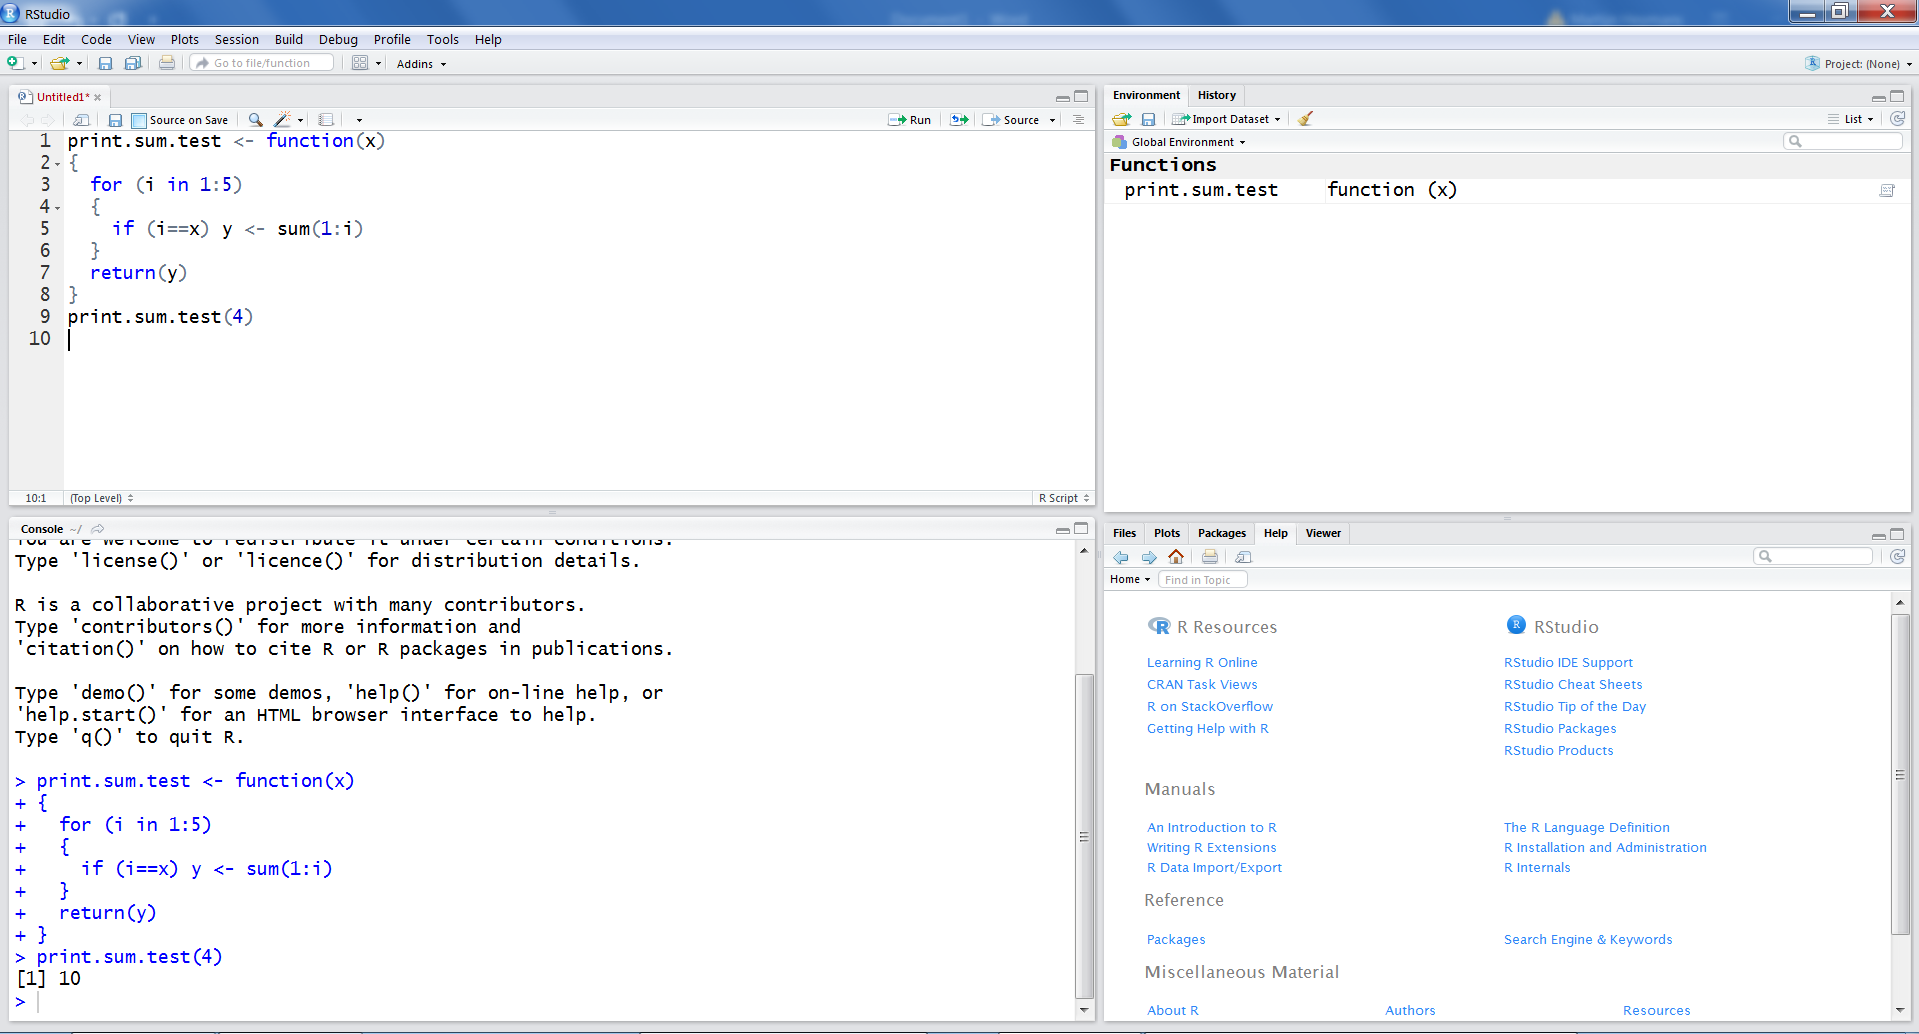
\includegraphics[width=0.9\linewidth]{images/fig1.11} 

}

\caption{Script file example in RStudio}\label{fig:fig11}
\end{figure}

\subsection{Creating a working
directory}\label{creating-a-working-directory}

It is a good idea to keep your R files at the same place when you are
doing data analysis for some kind of project. If you do not use a
separate directory, R will use a default directory, that will mostly be
in Windows in the documents folder. All files that you have to use
during your R session are assumed to be in that directory. Further, all
files that you save during your session will be in that directory. To
locate your working directory, you can type in the Console window:

If you want to change your working directory to for example
C:\Users\MWHeymans\Documents\R (Note that the path in R uses forward
slashes and the path in Windows backward slashes!), you can type:
\code{setwd("C:/Users/MWHeyamns/Documents/R")} \code{getwd()}

In Rstudio there is another way to get information about the current
working directory and another way to change the working directory. Go in
RStudio to the window on the right site below and go to the Files tab
and click on the right site of the screen on the three dots. Than a
window will open and you can browse to your preferred folder. Then
choose for More in the Files tab and then select ``Set As Working
Directory'' (Figure \ref{fig:fig12}). Now you have set your preferred
working directory. You can check if your directory is set correctly by
choosing ``Go To Working Directory''.

\begin{figure}

{\centering 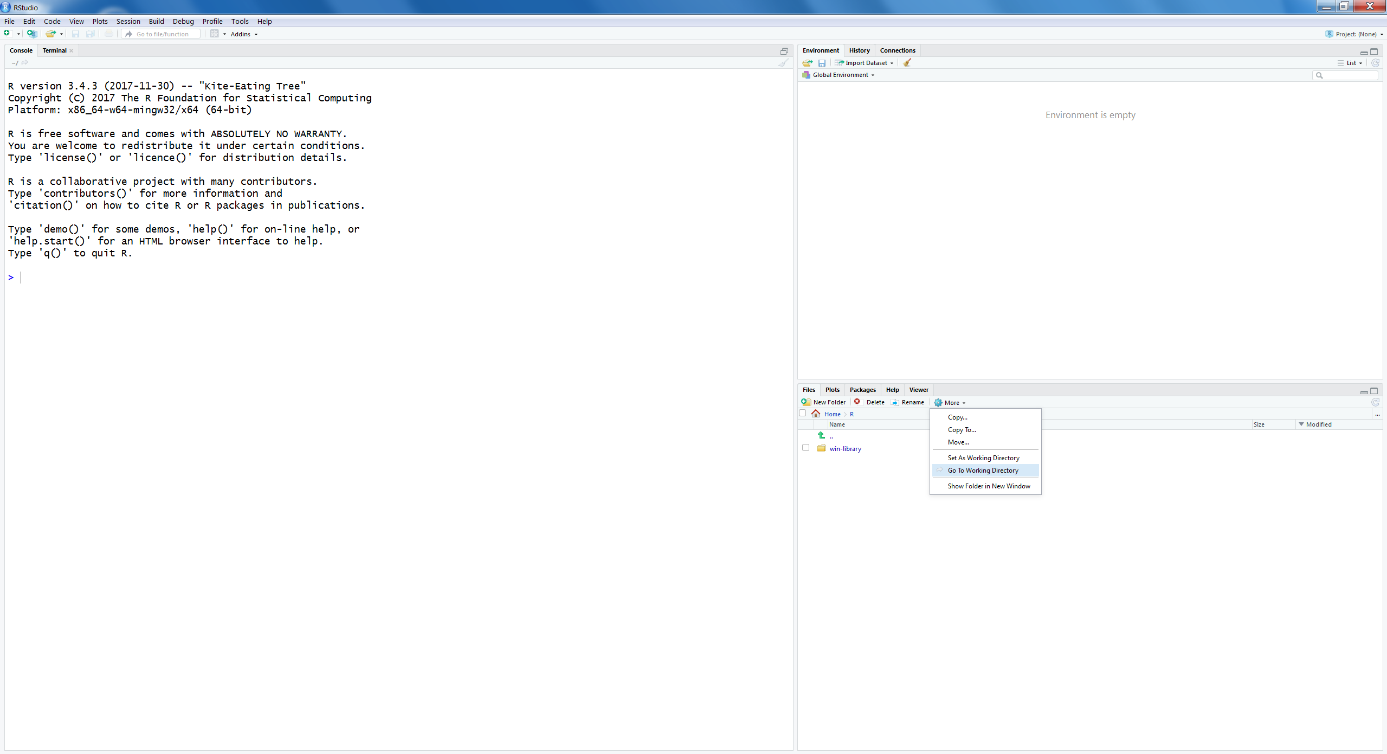
\includegraphics[width=0.9\linewidth]{images/fig1.12} 

}

\caption{Working directory selection in RStudio}\label{fig:fig12}
\end{figure}

\subsection{Reading in SPSS data in
RStudio}\label{reading-in-spss-data-in-rstudio}

There are several procedures in RStudio to read in datasets.

\begin{enumerate}
\def\labelenumi{\arabic{enumi}.}
\tightlist
\item
  Import datasets via ``Import Dataset'' An easy way to do that is via
  the window at the right site above. There you will find the button
  which is called ``Import Dataset''. When you click on it you can
  choose between different kind of file types, i.e.~CVS, Excel, SPSS,
  SAS and Stata files (Figure 1.13).
\end{enumerate}

\begin{figure}

{\centering 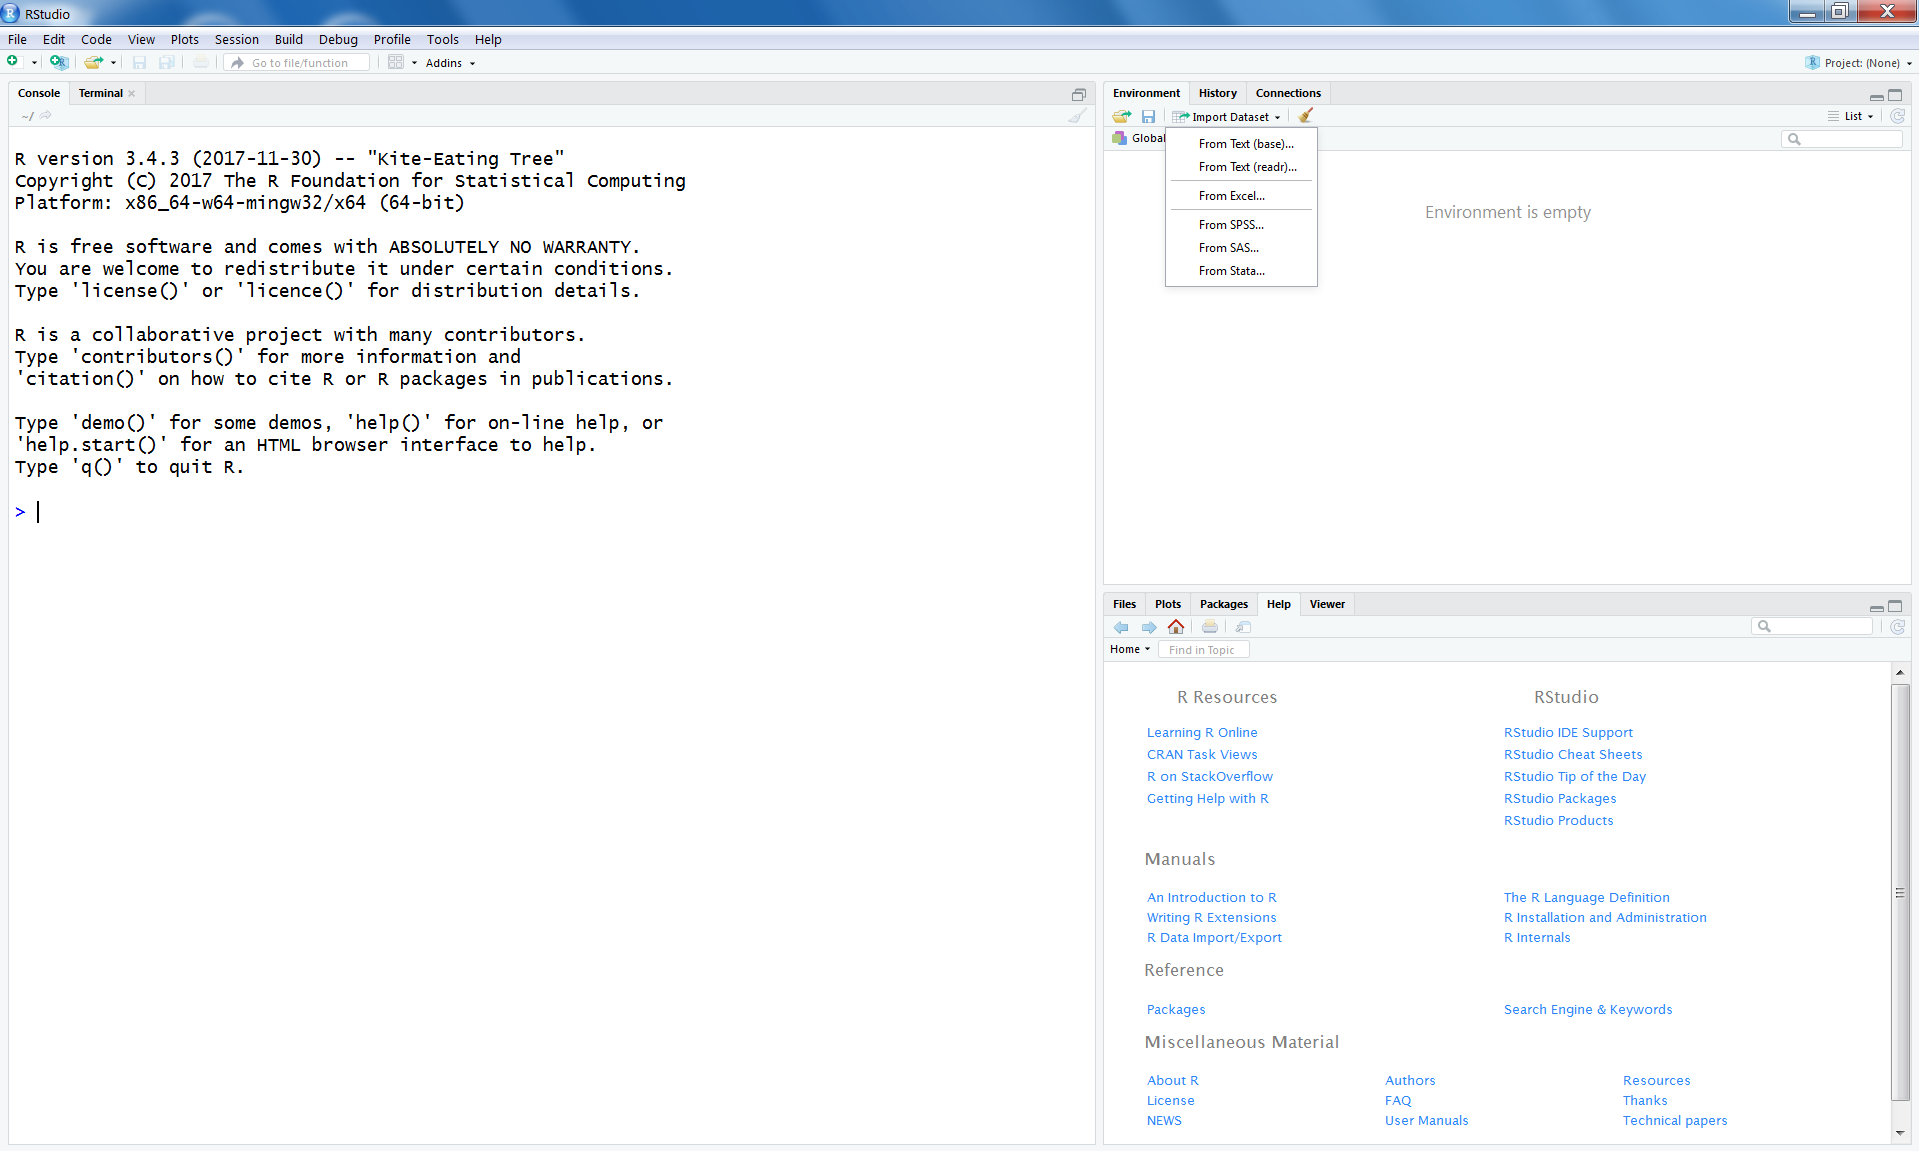
\includegraphics[width=0.9\linewidth]{images/fig1.13} 

}

\caption{Screen to import datasets in RStudio}\label{fig:fig13}
\end{figure}

In this example we choose for SPSS. When you approach this procedure for
the first time it could be that RStudio asks for your permission to
download a package called ``haven''. This package is built to import and
export data from several types. The following window will then appear
(Figure 1.14).

\begin{figure}

{\centering 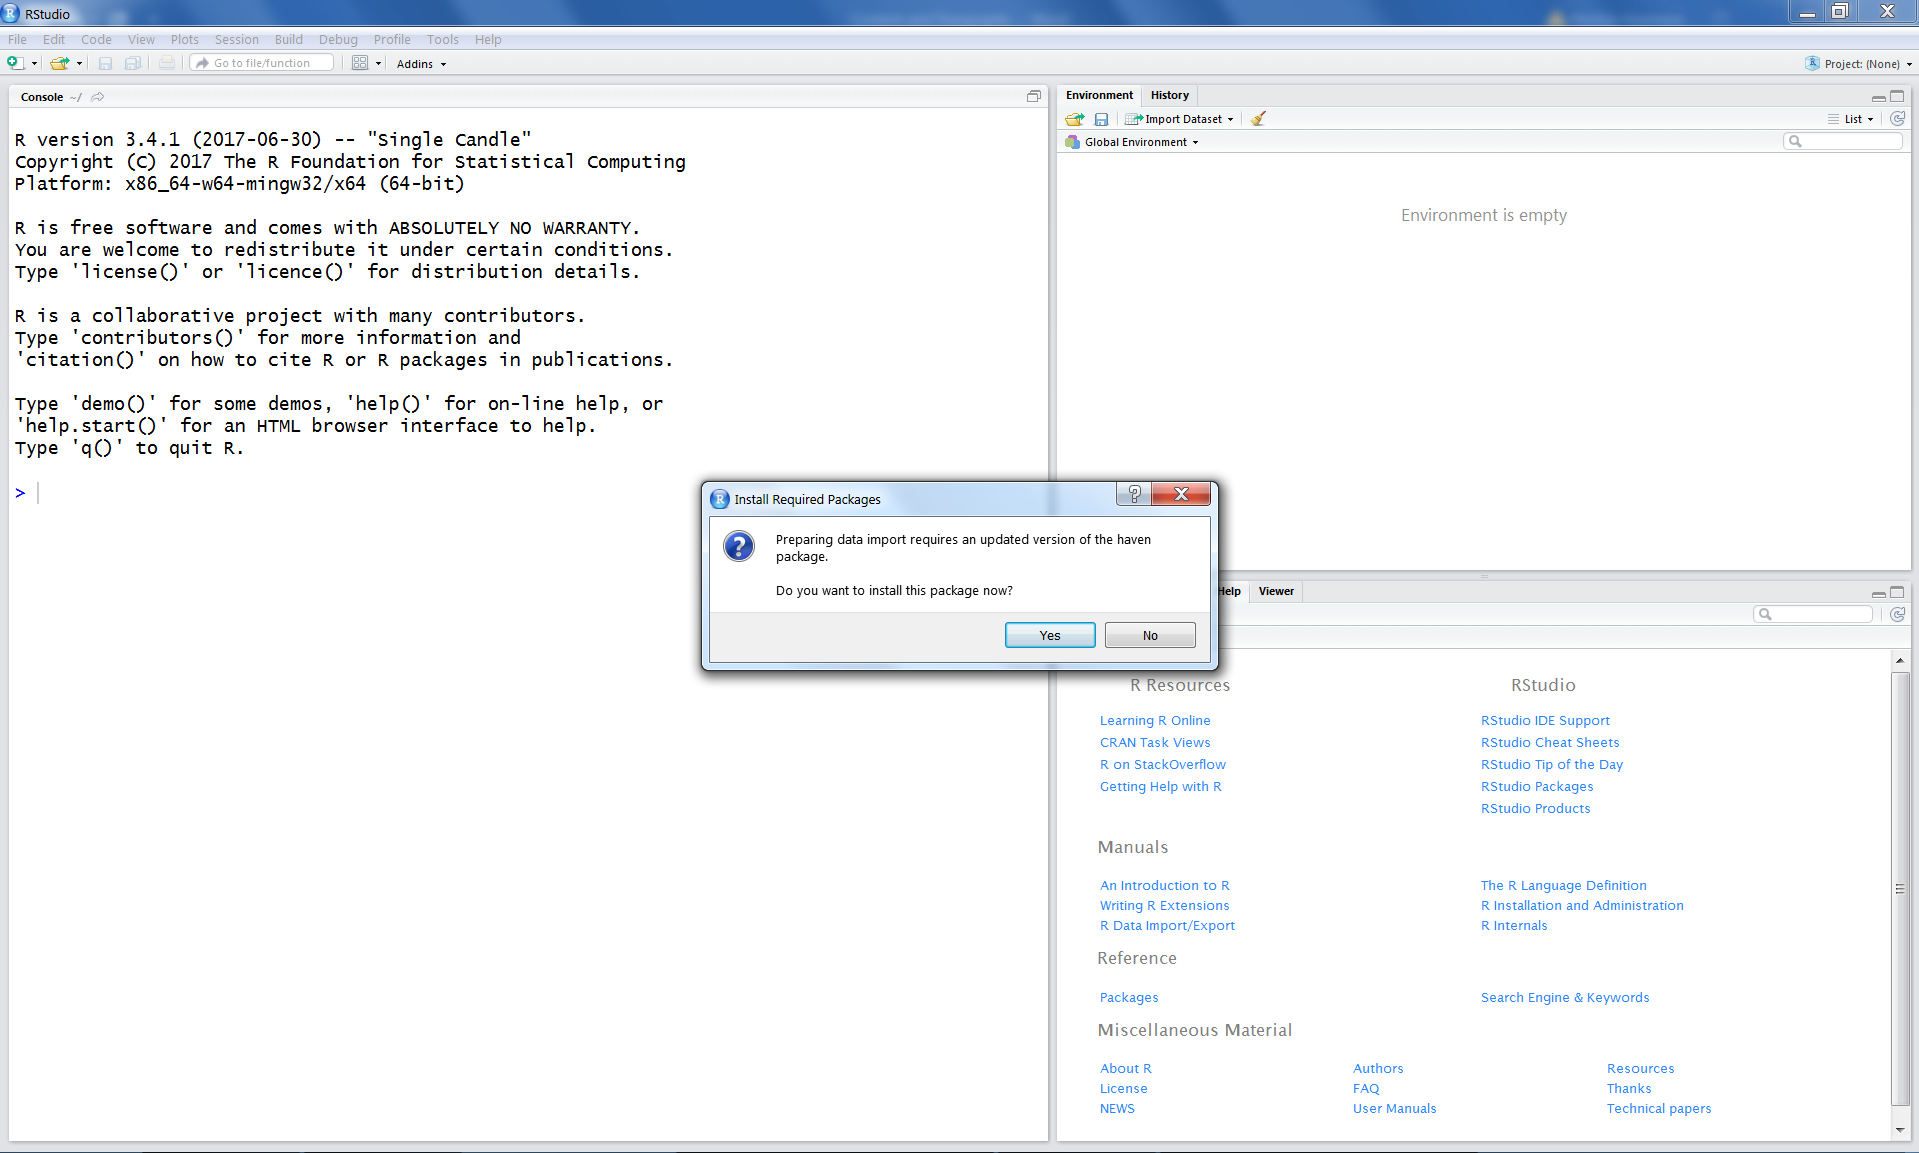
\includegraphics[width=0.9\linewidth]{images/fig1.14} 

}

\caption{Window to install the haven package}\label{fig:fig14}
\end{figure}

Click Yes and the download will start from the CRAN website. After the
package is installed a new window will open which is called ``Import
Statistical Data'' (Figure 1.15).

\begin{figure}

{\centering 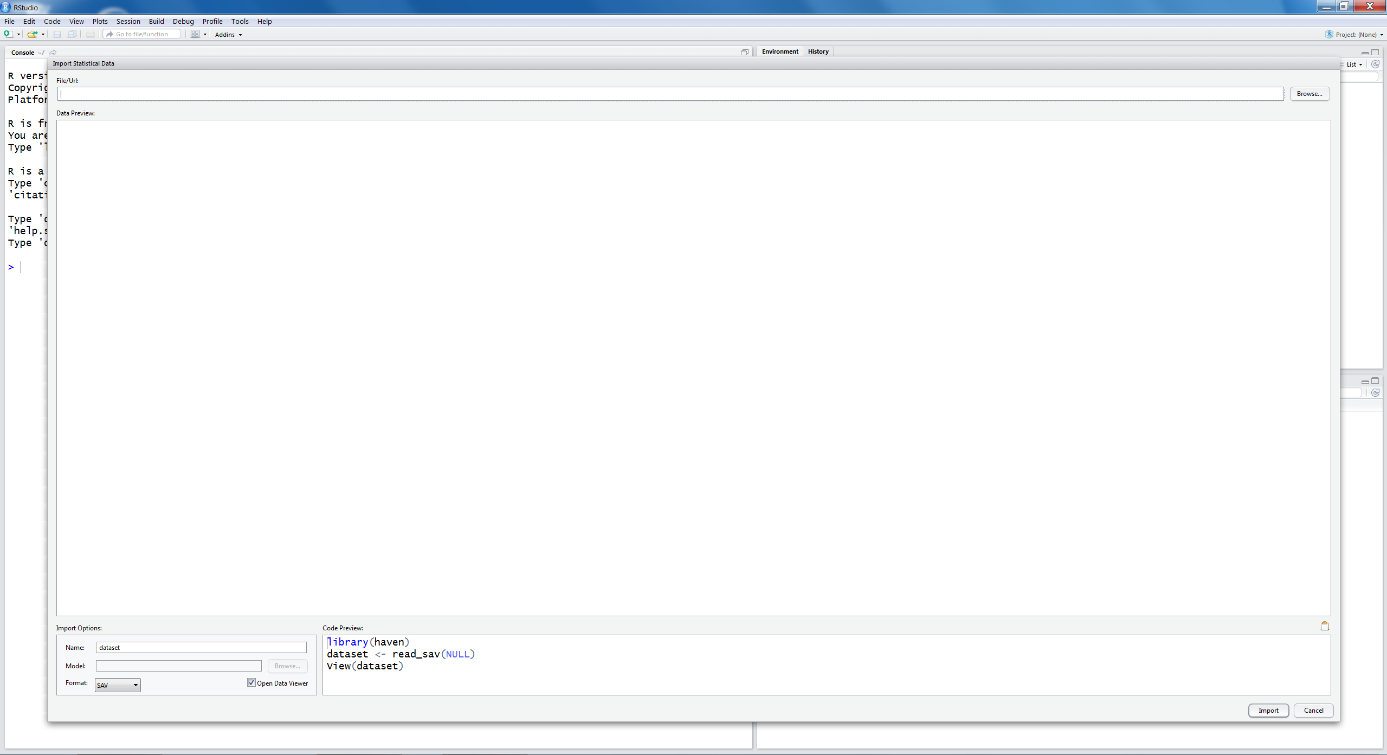
\includegraphics[width=0.9\linewidth]{images/fig1.15} 

}

\caption{The Import Statistical Data window in RStudio}\label{fig:fig15}
\end{figure}

At the top right site of the window you find the button which is called
``Browse''. That button allows you to browse to your dataset on your
computer. After you have opened your dataset you see a preview of your
dataset in RStudio (Figure 1.16).

\begin{figure}

{\centering 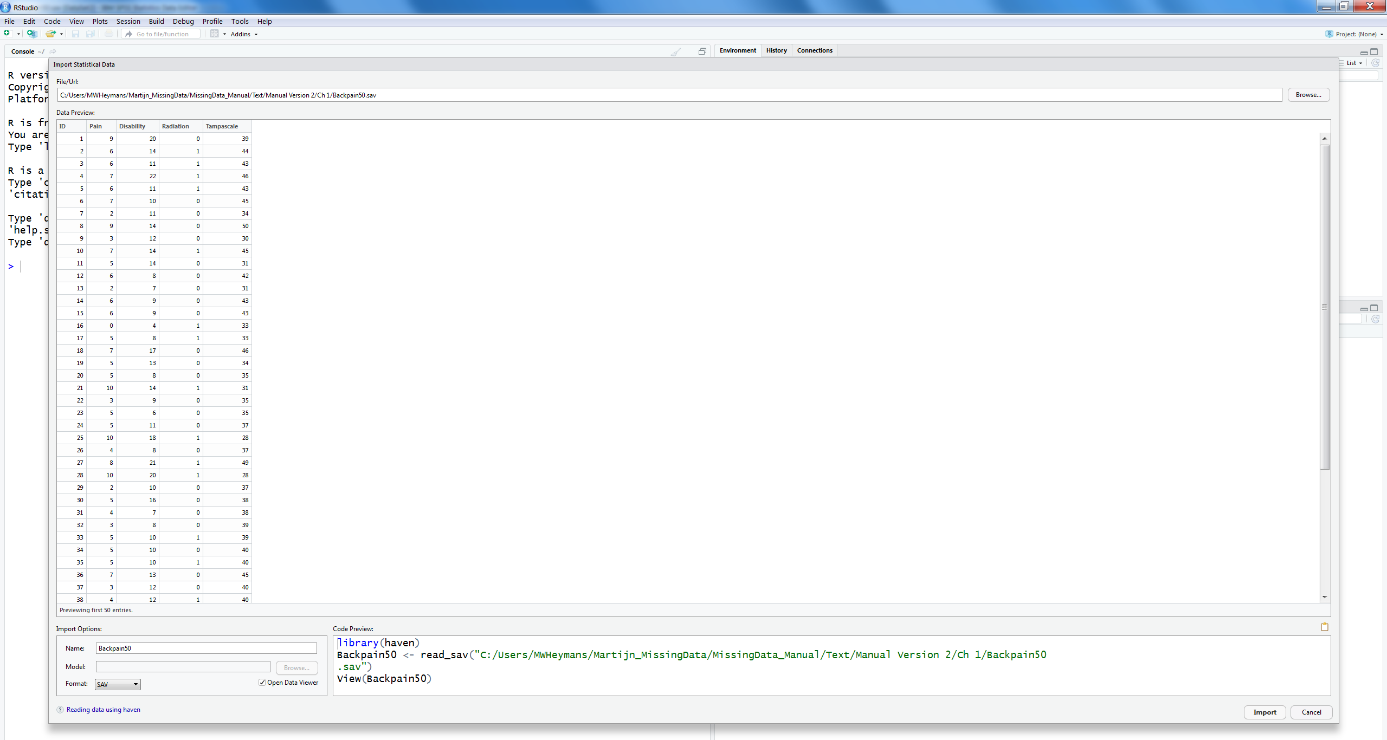
\includegraphics[width=0.9\linewidth]{images/fig1.16} 

}

\caption{A preview of the dataset in RStudio}\label{fig:fig16}
\end{figure}

Under Code Preview, under in the window, you see the code that was used
by RStudio to read in the dataset:

The dataset is automatically assigned to the object: Backpain50, which
is the original name of the dataset. When you click on Import, the
dataset is imported in the RStudio environment (Figure 1.17).

\begin{figure}

{\centering 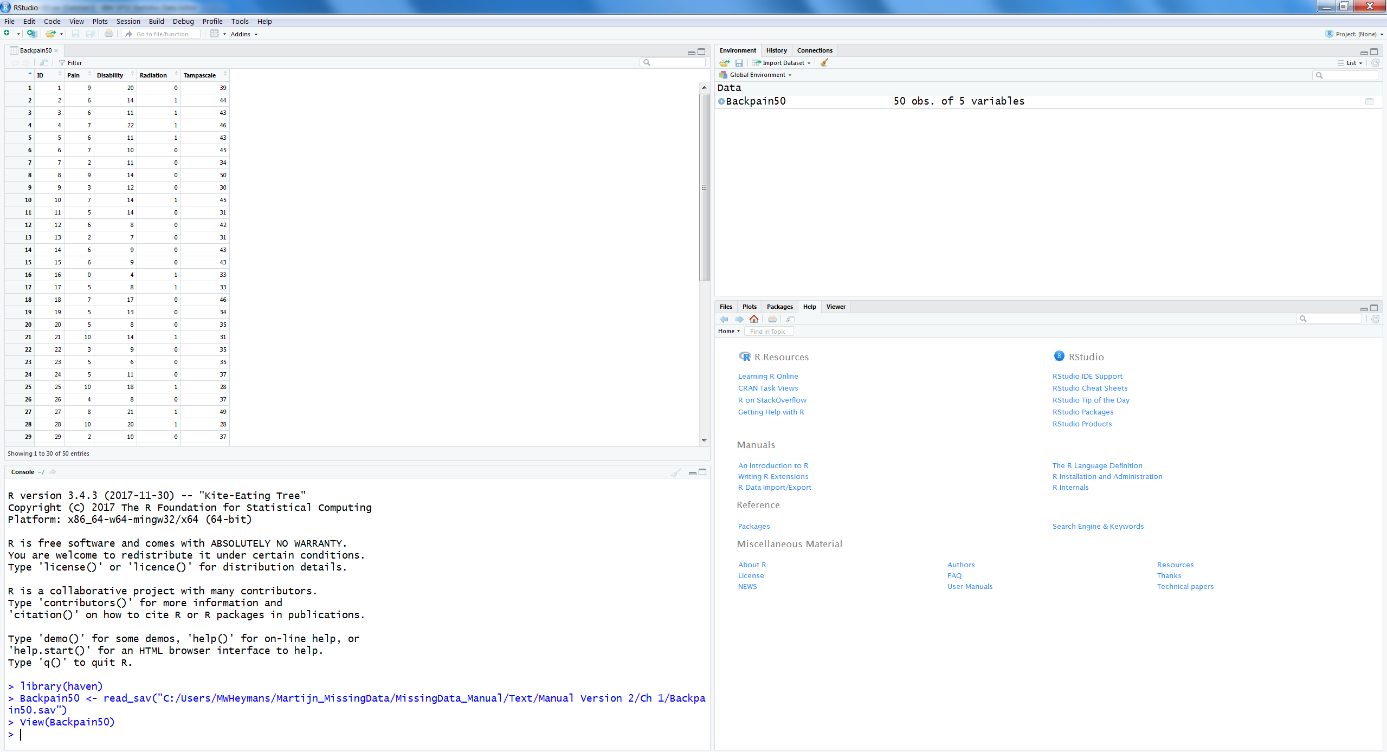
\includegraphics[width=0.9\linewidth]{images/fig1.17} 

}

\caption{Imported dataset in RStudio}\label{fig:fig17}
\end{figure}

Another way to import an SPSS dataset is by making use of the foreign
package. You can find this package under the Packages Tab in the window
at the right site below under the heading ``System Library''. Install
that package first. The foreign package includes the function
``read.spss''. Let's first explore the function arguments of this
function by using:

Now the following information can be found in the right window below,
under the Help tab:

read.spss(file, use.value.labels = TRUE, to.data.frame = FALSE,
max.value.labels = Inf, trim.factor.names = FALSE, trim\_values = TRUE,
reencode = NA, use.missings = to.data.frame)

The most important arguments to change for us are the file and
to.data.frame arguments. When you are in the correct working directory,
i.e.~the working directory where the file that you want to import is
stored, you use the following code to import the dataset:

\subsection{Saving and Reading R data in
RStudio}\label{saving-and-reading-r-data-in-rstudio}

Datasets can be saved and read in R using different commands.

\emph{Write.table} and \emph{Read.table}

\emph{Write.table} The write.table function can be used to write
matrices and data frames (datasets) to the working directory. The R code
is:

Files that have been written with write.table can be easily read in, in
SPSS by using the steps that will be discussed in the next paragraph.

\emph{Read.table} The read.table function can be used to read in
matrices and data frames by using:

\emph{Save and Load}

\emph{Save} You can also use the command save to save datasets,
according to (notice the .RData extension):

\emph{Load} Loading the dataset again in the workspace can be done by
using:

You can also use save by using the default options in the following way
to save your datasets:

To get direct access to the data that you have saved, you can use the
get function in combination with the load function like this:

With save, you can save any R object, also lists such as:

Subsequently, after you have removed object x from the workspace, you
can load it again by using:

\subsection{Reading in (R)Studio data into
SPSS}\label{reading-in-rstudio-data-into-spss}

When you have used the write.table function to save data in R you can
easily read them in into SPSS. First you have to use write.table in the
following way:

The extra parameter settings, mean: sep=``;'', separate each variable by
an ``;'' indicator. dec=``,'', use for decimals a ``,'' instead of an
``.''. row.names=F , Do not add an extra column with row.names.

Follow the next steps to read in the data into SPSS: choose File
-\textgreater{} Open data -\textgreater{} ``All files (\emph{.})'', than
you will see the file you want to read in into SPSS. In this example we
will use the file ``Backpain50 R file'' from R code 1.41 (Figure 1.18).

\begin{figure}

{\centering 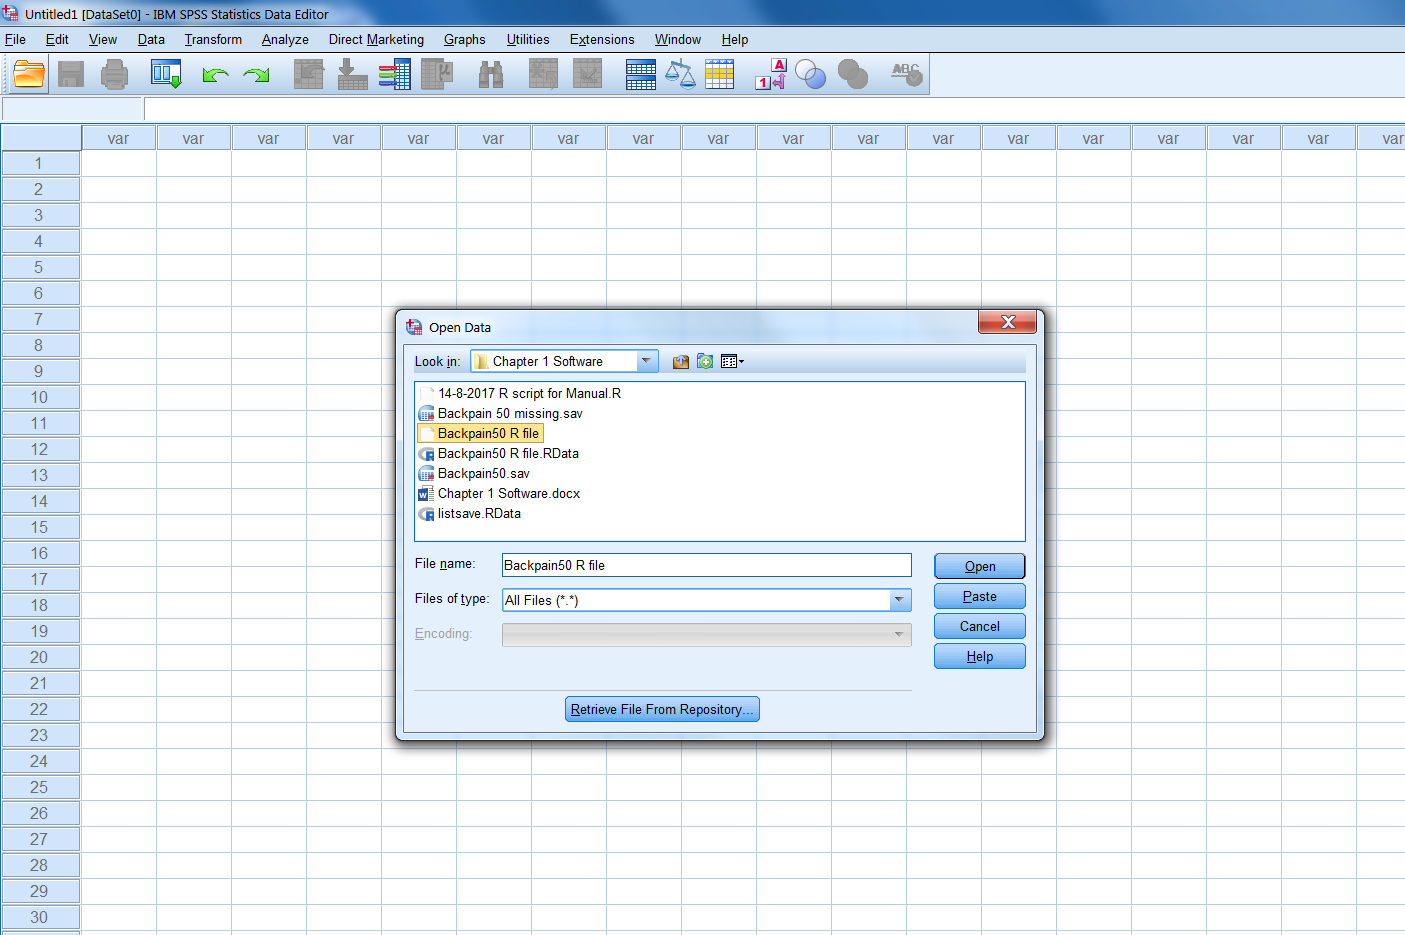
\includegraphics[width=0.9\linewidth]{images/fig1.18} 

}

\caption{Choosing the dataset to import in SPSS}\label{fig:fig18}
\end{figure}

Then click Open (wait a couple of seconds) and click on next. You will
see the following window that is part of the Text Import Wizard
procedure in SPSS (Figure 1.19):

\begin{figure}

{\centering 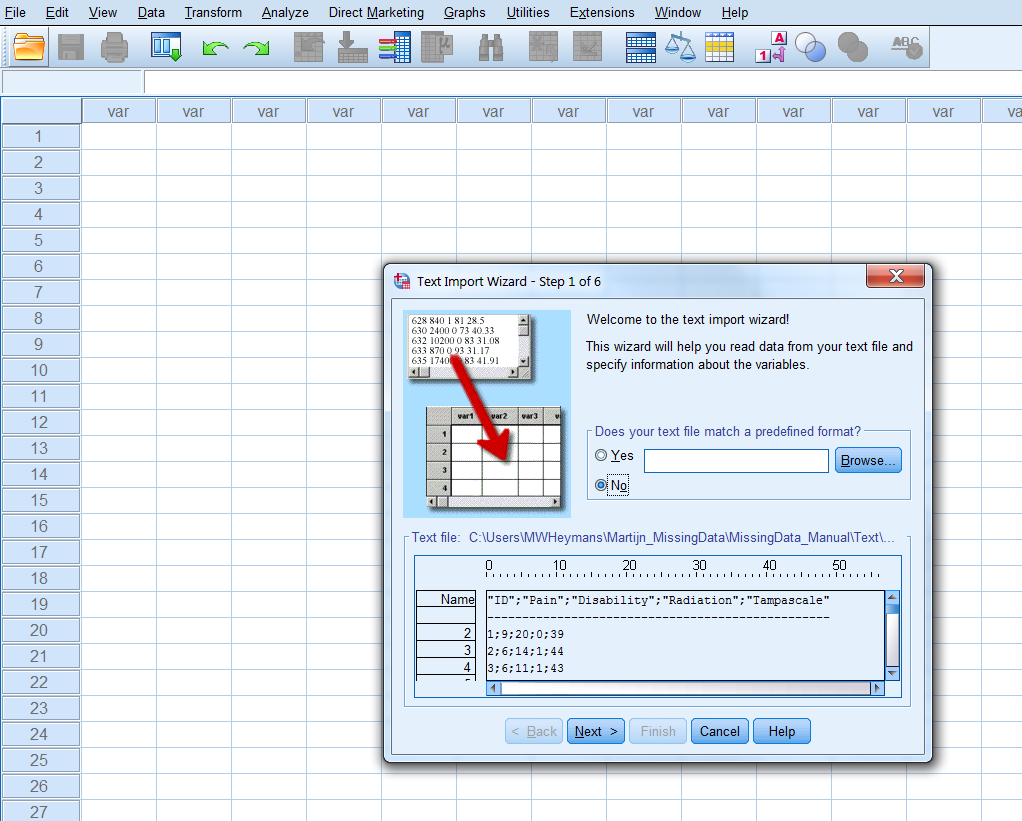
\includegraphics[width=0.9\linewidth]{images/fig1.19} 

}

\caption{Step 1 of the Text Import Wizard}\label{fig:fig19}
\end{figure}

Then click the ``Next \textgreater{}'' button 5 times, passing by the
following windows:

Step 2 of 6 (Figure 1.20): To change how variables are arranged: here
delimited To include variable names included at the top of the file:
here Yes. To set the decimal symbol: here a comma.

\begin{figure}

{\centering 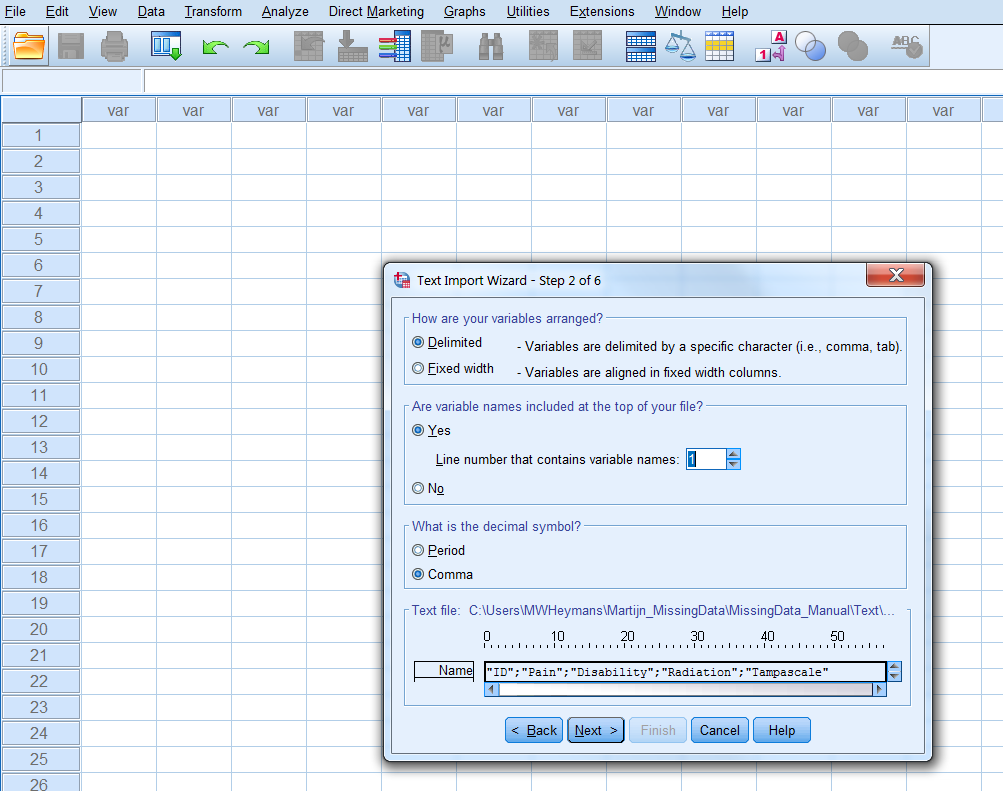
\includegraphics[width=0.9\linewidth]{images/fig1.20} 

}

\caption{Step 2 of the Text Import Wizard}\label{fig:fig20}
\end{figure}

Step 3 of 6 (Figure 1.21):

On which line number begins the first case: here 2 How cases are
represented: Each line is a case. How many cases you want to import:
here all cases.

\begin{figure}

{\centering 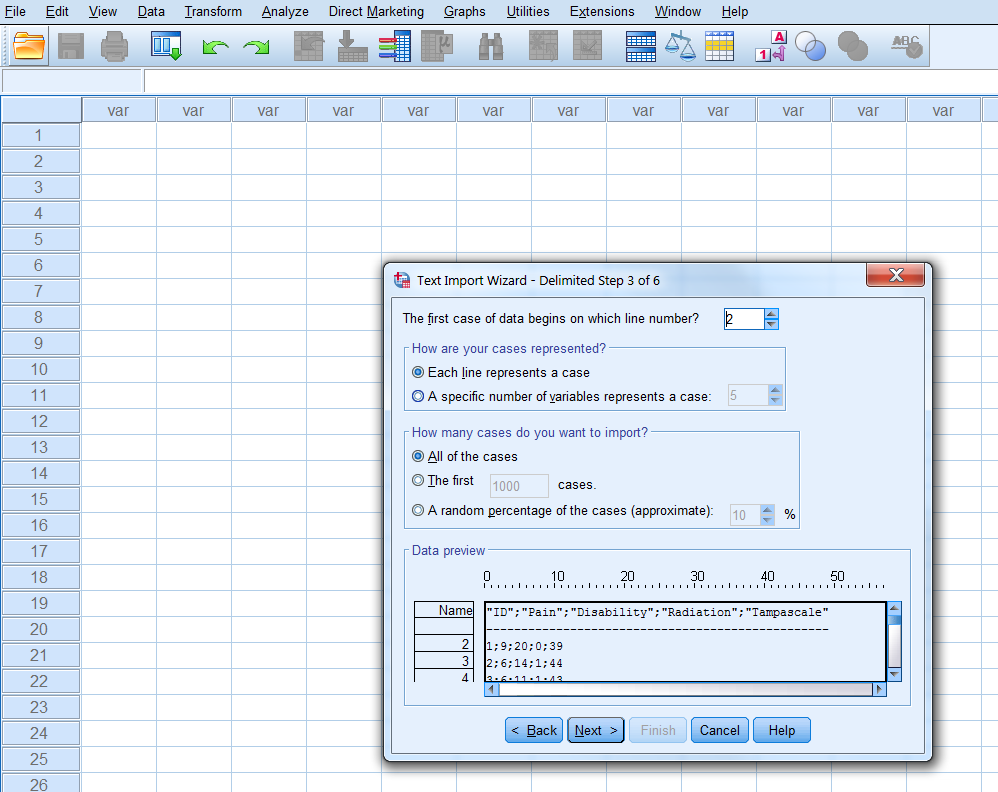
\includegraphics[width=0.9\linewidth]{images/fig1.21} 

}

\caption{Step 3 of the Text Import Wizard}\label{fig:fig21}
\end{figure}

Step 4 of 6 (Figure 1.22): The delimiters that appear between variables;
here the Semicolon. The text qualifier: here Double quote. Remove
trailing spaces from string values: skip.

\begin{figure}

{\centering 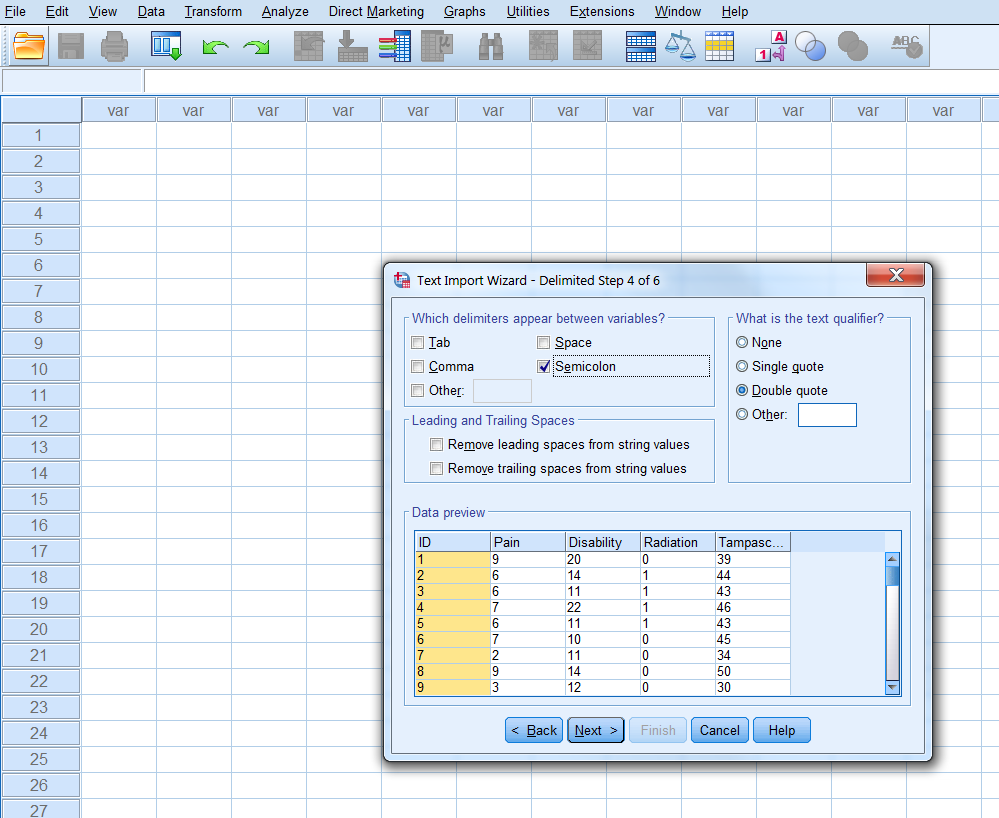
\includegraphics[width=0.9\linewidth]{images/fig1.22} 

}

\caption{Step 4 of the Text Import Wizard}\label{fig:fig22}
\end{figure}

Step 5 of 6 (Figure 1.23): Here you can overwrite the Data format of the
variable (you can also change that in the Variable View window, when the
data has been read in).

\begin{figure}

{\centering 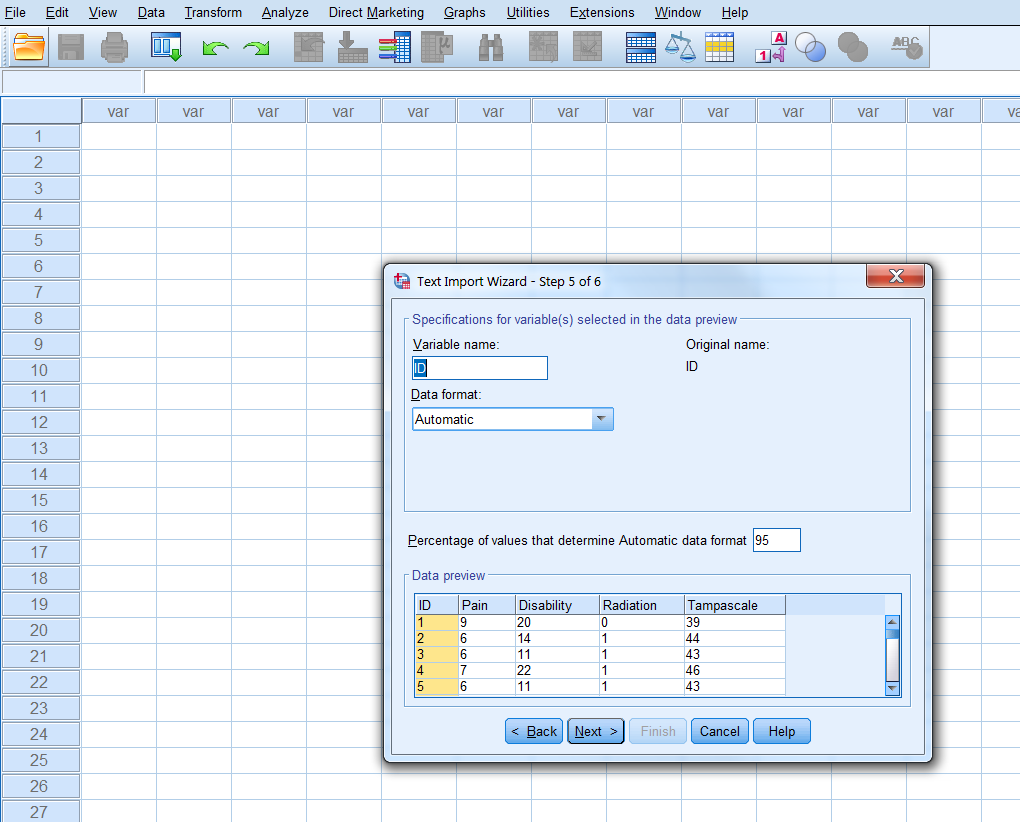
\includegraphics[width=0.9\linewidth]{images/fig1.23} 

}

\caption{Step 5 of the Text Import Wizard}\label{fig:fig23}
\end{figure}

Step 6 of 6: This step allows you to save your specifications of the
previous steps into a separate file (Figure 1.24).

\begin{figure}

{\centering 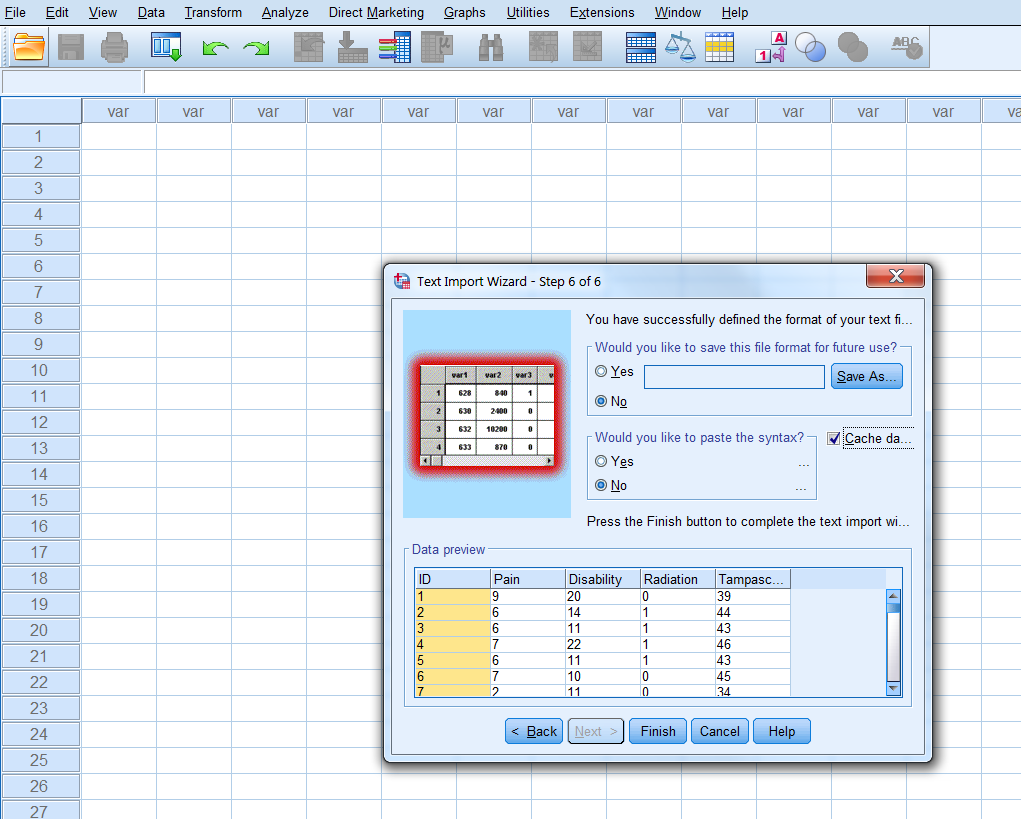
\includegraphics[width=0.9\linewidth]{images/fig1.24} 

}

\caption{Step 6 of the Text Import Wizard}\label{fig:fig24}
\end{figure}

Then click finish and the data will be read in, into a new SPSS file. In
that file you can of course change all kind of variable and data
settings in the Variable View Window.

You can also skip step 2 to 5 by clicking the Finish button twice when
you are at step 1. Than you use all default settings, which is most of
the times a good option.

\subsection{Installing R Packages}\label{installing-r-packages}

When R is installed on your computer also a folder called library is
created. This folder contains packages that are part of the basic
installation. A package is a collection of different functions written
in the R language. Besides packages that are part of the basic
installation of R there are also packages that are not part of the basic
installation but are written by others, i.e.~the add-on packages.
Packages can be downloaded from the CRAN website
(\url{https://cran.r-project.org/}). Currently, there are thousands of
user-written packages available on the CRAN website.

Before you can use a specific package that is not part of the basic
installation, you have to install it in your R library. In this manual
we will use the mice package to do all kind of imputation procedures,
such as multiple imputation. mice is not part of the basic installation
so we have to install it first. There are several procedures in RStudio
to install a package. One way is to use the install.packages function in
the Console window as follows:

The mice package will be automatically downloaded from the CRAN website.

Another way is to use the window on the right site below and go to the
Packages tab. When you click ``Install'' a new window is opened. Than
you can type ``mice'' on the blank line under ``Packages (separate
multiple with space or comma):'' (Figure 1.25a and b).

\begin{figure}

{\centering 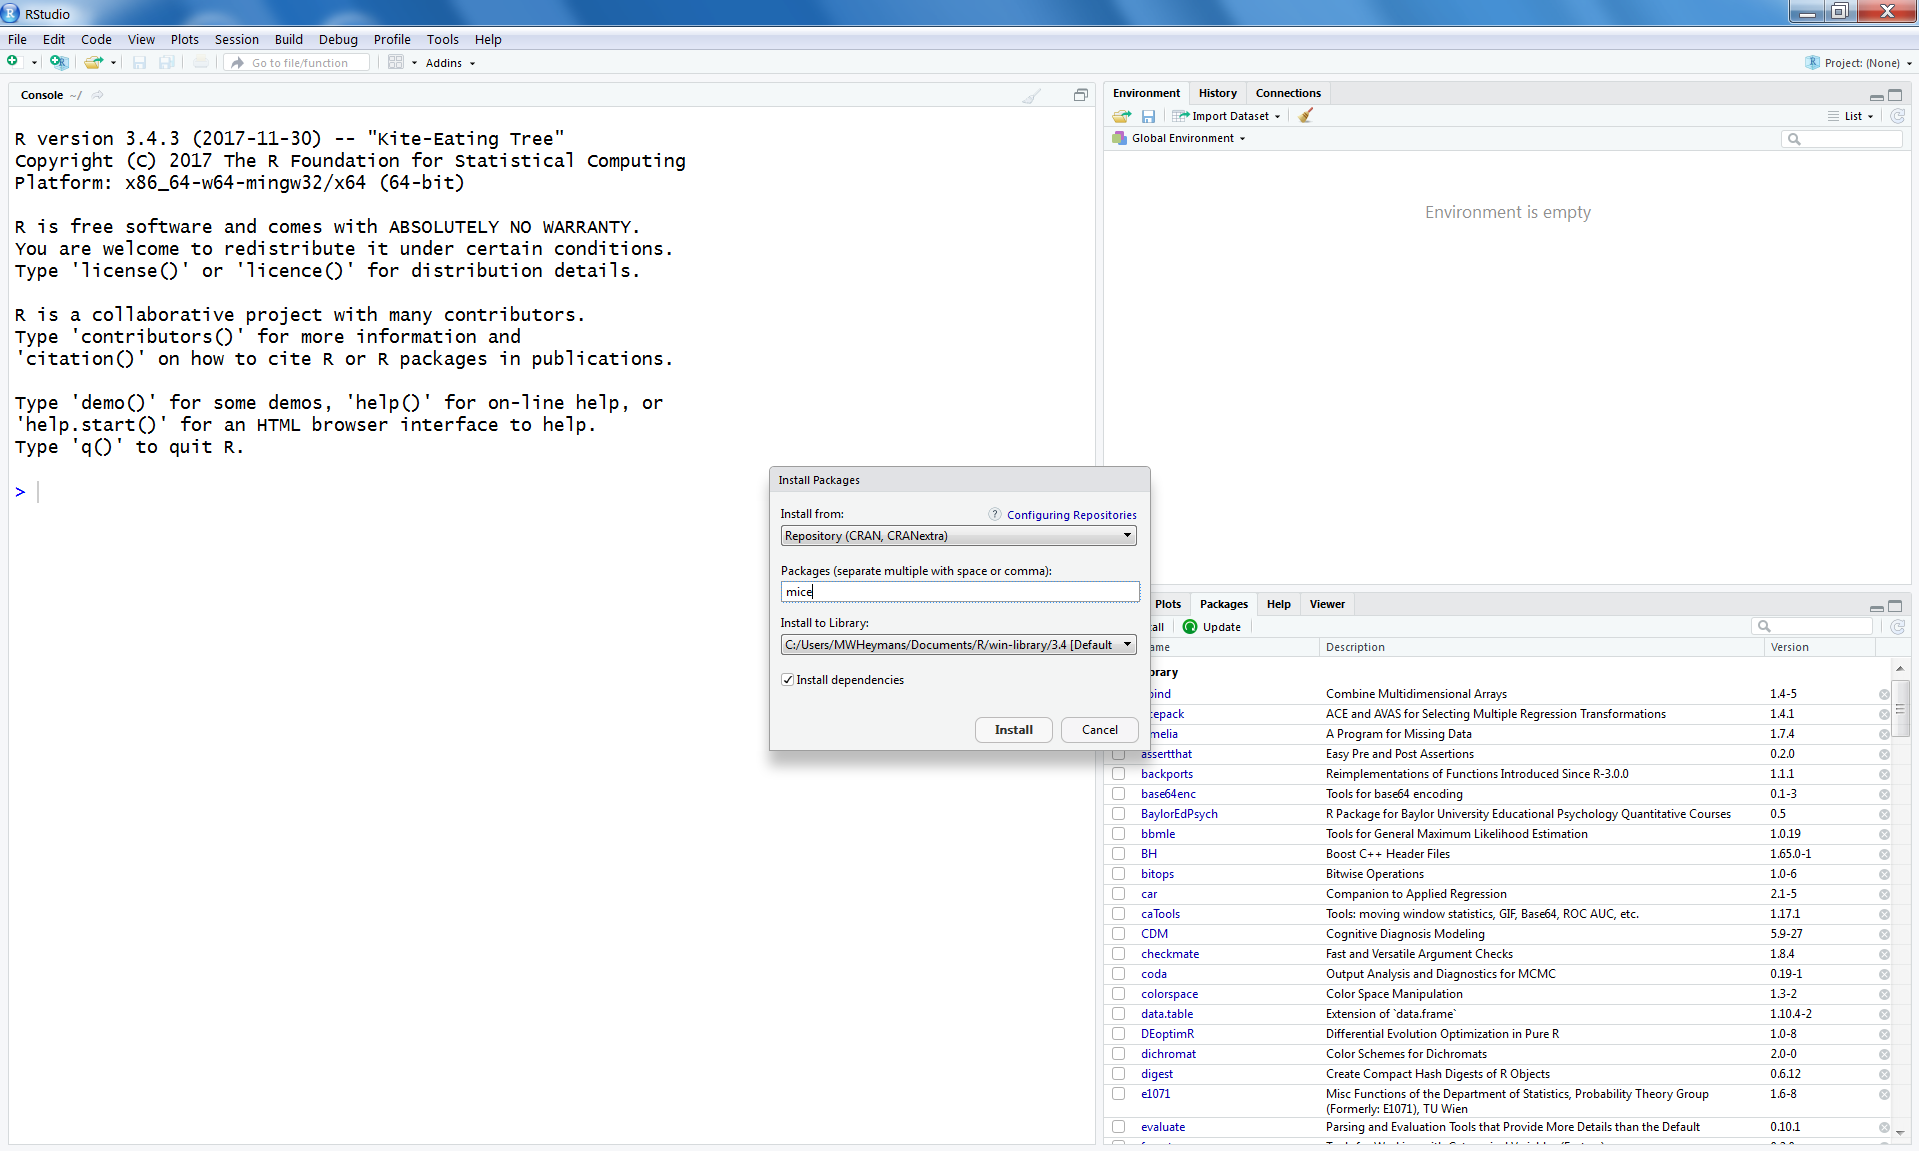
\includegraphics[width=0.9\linewidth]{images/fig1.25a} 

}

\caption{Install packages Window in RStudio to install packages from the CRAN website}\label{fig:fig25a}
\end{figure}

\begin{figure}

{\centering 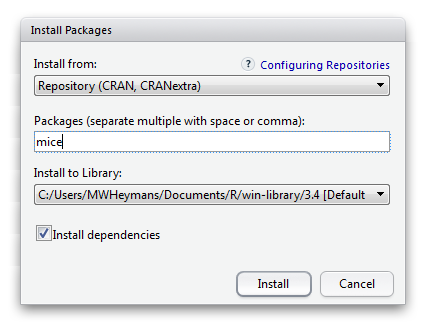
\includegraphics[width=0.9\linewidth]{images/fig1.25b} 

}

\caption{Enlarged Install packages Window in RStudio to install packages from the CRAN website}\label{fig:fig25b}
\end{figure}

After you have clicked on ``Install'' the package will be downloaded
from the CRAN website automatically and will be listed in the Package
list named ``User Library''.

Another way is to go to the CRAN website and download the package as a
zip file in a directory on your computer, for example your working
directory or in your library. Again use the window on the right site
below and go to the Packages tab. When you choose Install a new window
is opened. Now under ``Install from:'' choose for ``Package Archive File
(.zip; .tar.gz)'' (Figure 1.26a and 1.26b). Than you can browse to the
zip file and install the package.

\begin{figure}

{\centering 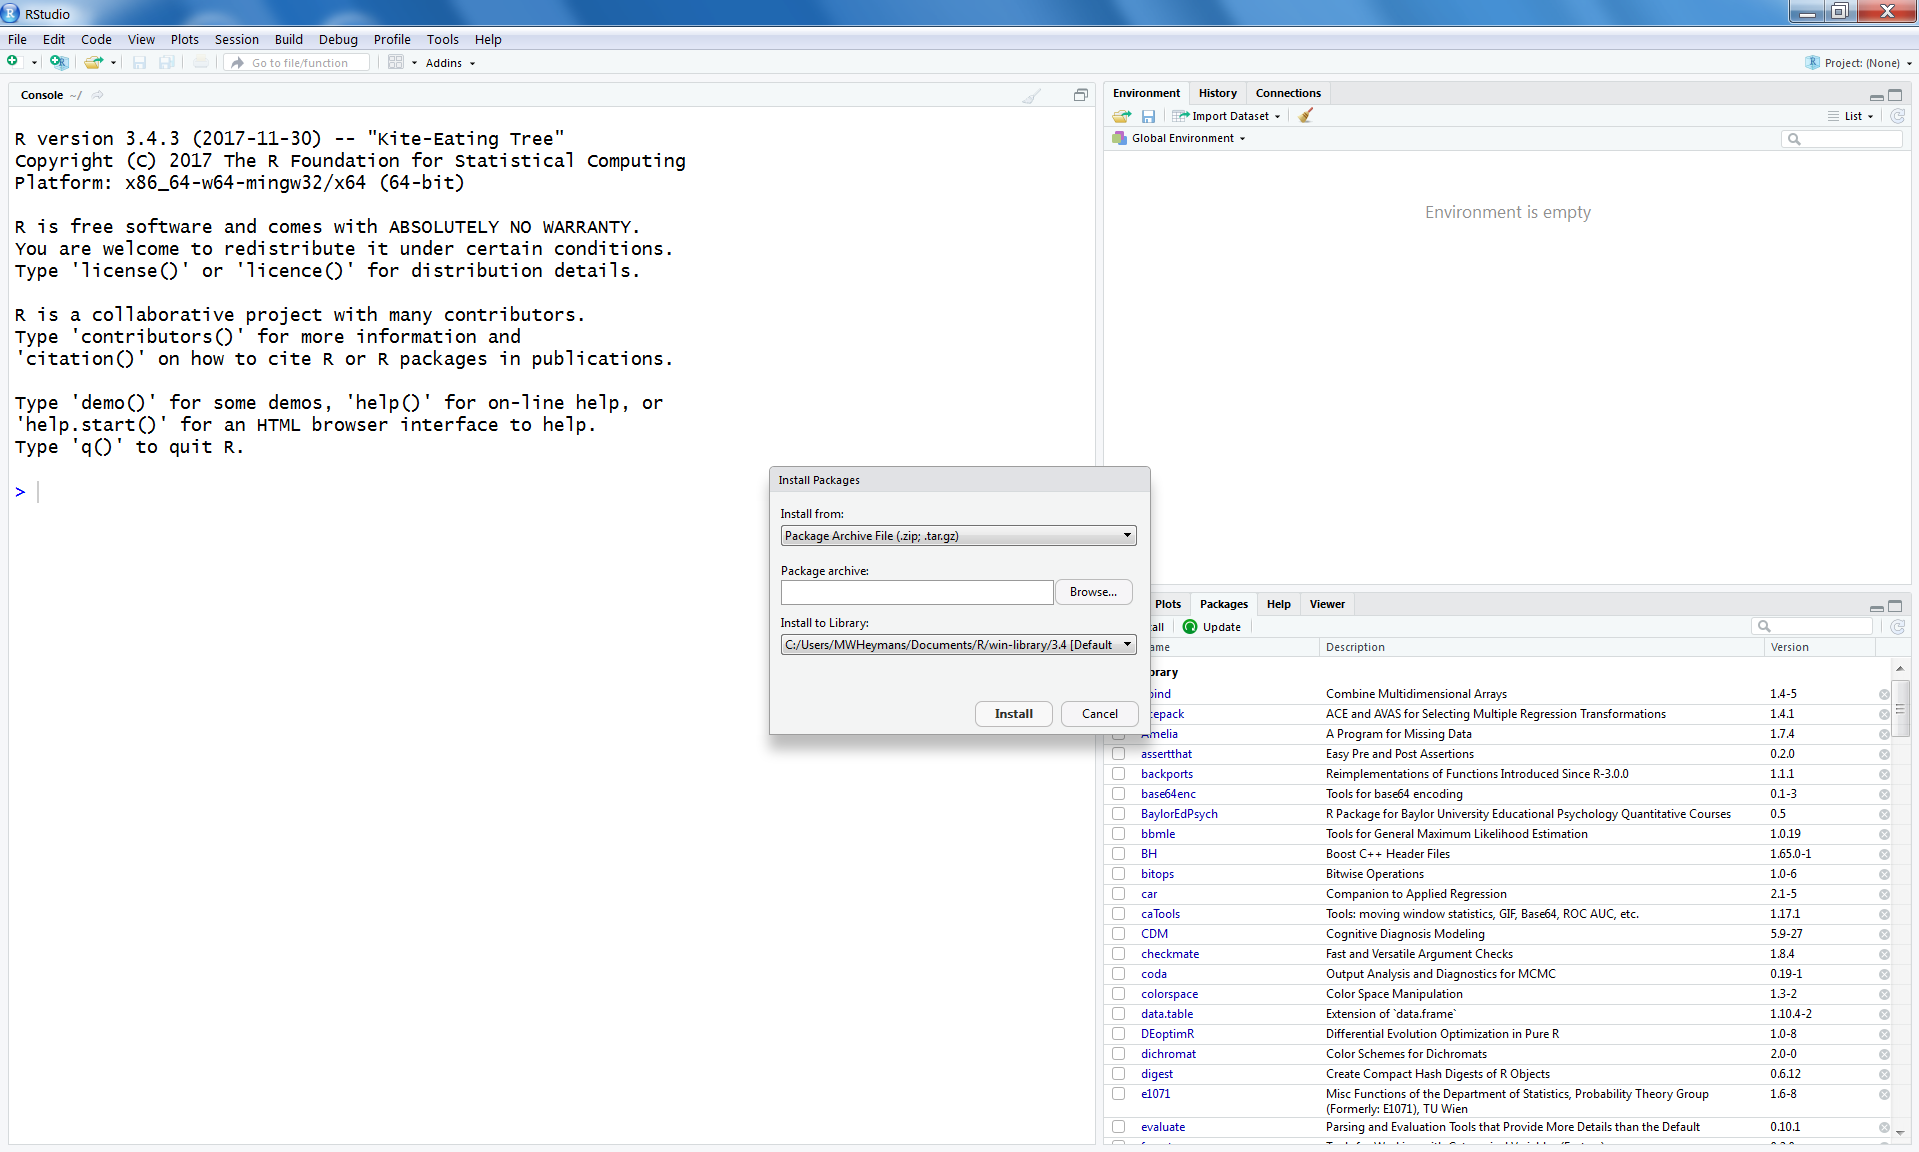
\includegraphics[width=0.9\linewidth]{images/fig1.26a} 

}

\caption{Install packages Window in RStudio to install packages from zip files}\label{fig:fig26a}
\end{figure}

\begin{figure}

{\centering 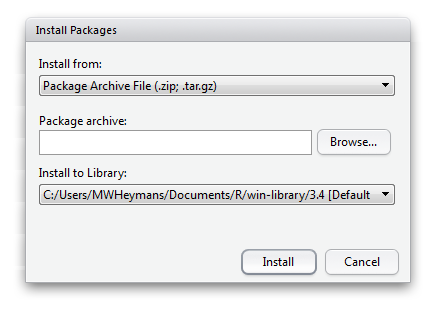
\includegraphics[width=0.9\linewidth]{images/fig1.26b} 

}

\caption{Enlarged Install packages Window in RStudio to install packages from zip files}\label{fig:fig26b}
\end{figure}

\subsection{Loading R Packages}\label{loading-r-packages}

Once an add-on (user written) R package has been installed it has to be
loaded to get access to all functions that are part of that package. To
load a library, you can use the function library() or require(). R code
1.43 shows an example of loading the mice package.

The require() function is used in the same way. You have to load add-on
packages each time you start a new R session.

\subsection{Updating R Packages}\label{updating-r-packages}

To keep the add-on packages up to date you can use the update.packages()
function in R. R code 1.44 presents an example.

R will ask you if you want to update each package. If you type ``y'' in
the Console window, R will update the package.

In RStudio updating packages can be done in the Package tab as well. You
can click on the Update button. A new window will open that contains a
list of all packages that need to be updated. Subsequently you can
select the packages you want to update.

\subsection{Useful Missing data Packages and
links}\label{useful-missing-data-packages-and-links}

The main package that we will use in this manual is mice which stand for
Multivariate Imputation by Chained Equations (MICE) (Van Buuren, 2009).

Other packages that are related to MICE are miceadds and micemd:
miceadds: this package contains some additional multiple imputation
functions (Robitzsch et al., 2017). See for more information:
\href{https://cran.r-project.org/web/packages/miceadds/index.html}{linked
phrase}

micemd: this package contains additional functions for the mice package
to perform multiple imputation in two-level (Multilevel) data (Audigier
\& Resche-Rigon, 2017). See for more information:
\href{https://cran.r-project.org/web/packages/micemd/index.html}{linked
phrase}

mi: provides functions for data manipulation, imputing missing values in
an approximate Bayesian framework, diagnostics of the models used to
generate the imputations, confidence-building mechanisms to validate
some of the assumptions of the imputation algorithm, and functions to
analyze multiply imputed data sets (Gelman et al., 2015). See for more
information:
\href{https://cran.r-project.org/web/packages/mi/index.html}{linked
phrase}

MItools: small package to perform analyses and combine results from
multiple-imputation datasets (Lumley, 2015). See for more information:
\href{https://cran.r-project.org/web/packages/mitools/index.html}{linked
phrase}

norm: this package is for the Analysis of multivariate normal datasets
with missing values. It contains the mi.inference function. This
function combines estimates and standard errors to produce a single
inference. Uses the technique described by Rubin (1987), which are
called the Rubin's Rules (RR) (Novo, 2015). See for more information:
\href{https://cran.r-project.org/web/packages/norm/index.html}{linked
phrase}

vim (visualization and imputation of missing values): This package
includes tools for the visualization of missing and/or imputed values.
In addition, the quality of imputation can be visually explored using
various univariate, bivariate, multiple and multivariate plot methods
(Templ et al., 2017). See for more information:
\href{https://cran.r-project.org/web/packages/mi/index.html}{linked
phrase}

BaylorEdPsych: R Package for Baylor University Educational Psychology
Quantitative Courses. This package included Little's MCAR test
(Beaujean, 2015). See for more information:
\href{https://cran.r-project.org/web/packages/BaylorEdPsych/index.html}{linked
phrase}

MKmisc: Contains several functions for statistical data analysis;
e.g.~for sample size and power calculations, computation of confidence
intervals, and generation of similarity matrices. This package contains
the mi.t.test function for pooling t-tests after multiple imputation
(Kohl, 2016). See for more information:
\href{https://cran.r-project.org/web/packages/MKmisc/index.html}{linked
phrase}

mvnmle: This package estimates the maximum likelihood estimate of the
mean vector and variance-covariance matrix for multivariate normal data
with missing values. This package is needed for the mlest function this
is used for Little's MCAR test in Cahpter 2. See for more information:
\href{https://cran.r-project.org/web/packages/mvnmle/index.html}{linked
phrase}

\bibliography{book.bib,packages.bib}


\end{document}
